% Options for packages loaded elsewhere
\PassOptionsToPackage{unicode}{hyperref}
\PassOptionsToPackage{hyphens}{url}
\PassOptionsToPackage{dvipsnames,svgnames,x11names}{xcolor}
%
\documentclass[
  10pt,
]{article}
\usepackage{amsmath,amssymb}
\usepackage{iftex}
\ifPDFTeX
  \usepackage[T1]{fontenc}
  \usepackage[utf8]{inputenc}
  \usepackage{textcomp} % provide euro and other symbols
\else % if luatex or xetex
  \usepackage{unicode-math} % this also loads fontspec
  \defaultfontfeatures{Scale=MatchLowercase}
  \defaultfontfeatures[\rmfamily]{Ligatures=TeX,Scale=1}
\fi
% lmodern omitted
\ifPDFTeX\else
  % xetex/luatex font selection
  \setmainfont[]{DejaVu Serif}
  \setsansfont[]{DejaVu Sans}
  \setmonofont[]{DejaVu Sans Mono}
  \setmathfont[]{DejaVu Math TeX Gyre}
\fi
% Use upquote if available, for straight quotes in verbatim environments
\IfFileExists{upquote.sty}{\usepackage{upquote}}{}
\IfFileExists{microtype.sty}{% use microtype if available
  \usepackage[]{microtype}
  \UseMicrotypeSet[protrusion]{basicmath} % disable protrusion for tt fonts
}{}
\makeatletter
\@ifundefined{KOMAClassName}{% if non-KOMA class
  \IfFileExists{parskip.sty}{%
    \usepackage{parskip}
  }{% else
    \setlength{\parindent}{0pt}
    \setlength{\parskip}{6pt plus 2pt minus 1pt}}
}{% if KOMA class
  \KOMAoptions{parskip=half}}
\makeatother
\usepackage{xcolor}
\usepackage[margin=2.2cm]{geometry}
\usepackage{longtable,booktabs,array}
\usepackage{calc} % for calculating minipage widths
% Correct order of tables after \paragraph or \subparagraph
\usepackage{etoolbox}
\makeatletter
\patchcmd\longtable{\par}{\if@noskipsec\mbox{}\fi\par}{}{}
\makeatother
% Allow footnotes in longtable head/foot
\IfFileExists{footnotehyper.sty}{\usepackage{footnotehyper}}{\usepackage{footnote}}
\makesavenoteenv{longtable}
\usepackage{graphicx}
\makeatletter
\def\maxwidth{\ifdim\Gin@nat@width>\linewidth\linewidth\else\Gin@nat@width\fi}
\def\maxheight{\ifdim\Gin@nat@height>\textheight\textheight\else\Gin@nat@height\fi}
\makeatother
% Scale images if necessary, so that they will not overflow the page
% margins by default, and it is still possible to overwrite the defaults
% using explicit options in \includegraphics[width, height, ...]{}
\setkeys{Gin}{width=\maxwidth,height=\maxheight,keepaspectratio}
% Set default figure placement to htbp
\makeatletter
\def\fps@figure{htbp}
\makeatother
\setlength{\emergencystretch}{3em} % prevent overfull lines
\providecommand{\tightlist}{%
  \setlength{\itemsep}{0pt}\setlength{\parskip}{0pt}}
\setcounter{secnumdepth}{-\maxdimen} % remove section numbering
\ifLuaTeX
\usepackage[bidi=basic]{babel}
\else
\usepackage[bidi=default]{babel}
\fi
\babelprovide[main,import]{czech}
\ifPDFTeX
\else
\babelfont{rm}[]{DejaVu Serif}
\fi
% get rid of language-specific shorthands (see #6817):
\let\LanguageShortHands\languageshorthands
\def\languageshorthands#1{}
\usepackage{caption}
\captionsetup{labelformat=empty,font=small}
\usepackage{float}
\floatplacement{figure}{H}
\usepackage{needspace}
\usepackage{etoolbox}
\pretocmd{\section}{\Needspace{10\baselineskip}}{}{}
\pretocmd{\subsection}{\Needspace{7\baselineskip}}{}{}
\usepackage{lastpage}
\usepackage{fancyhdr}
\fancypagestyle{plain}{\fancyhf{}\renewcommand{\headrulewidth}{0pt}\fancyfoot[C]{\small\thepage\,/\,\pageref*{LastPage}}}
\pagestyle{plain}
\widowpenalty=10000
\clubpenalty=10000
\renewcommand{\abstractname}{Abstrakt}
\ifLuaTeX
  \usepackage{selnolig}  % disable illegal ligatures
\fi
\IfFileExists{bookmark.sty}{\usepackage{bookmark}}{\usepackage{hyperref}}
\IfFileExists{xurl.sty}{\usepackage{xurl}}{} % add URL line breaks if available
\urlstyle{same}
\hypersetup{
  pdftitle={Hodnoty kvadratických Dirichletových L-funkcí ve středu pro
všechny fundamentální diskriminanty do 10\^{}7 a u 10\^{}8, 10\^{}9 a
10\^{}10: momenty, souvislé rodiny, rozdělení hodnot, první nula a
vážená hustota nízkých nul - reprodukovatelná numerická studie V},
  pdfauthor={David Hess (MAYAN ALFA V1008 LAB v.34.85b)},
  pdflang={cs},
  colorlinks=true,
  linkcolor={Maroon},
  filecolor={Maroon},
  citecolor={Blue},
  urlcolor={Blue},
  pdfcreator={LaTeX via pandoc}}

\title{Hodnoty kvadratických Dirichletových L-funkcí ve středu pro
všechny fundamentální diskriminanty do \(10^7\) a u \(10^8\), \(10^9\) a
\(10^{10}\): momenty, souvislé rodiny, rozdělení hodnot, první nula a
vážená hustota nízkých nul --- reprodukovatelná numerická studie V}
\author{David Hess (MAYAN ALFA V1008 LAB v.34.85b)}
\date{15.11.2026}

\begin{document}
\maketitle
\begin{abstract}
Pátá studie této řady přechází od nul kvadratických Dirichletových
L-funkcí (studie III) k jejich hodnotám ve středu kritického pásu.
Hodnoty \(L(\tfrac12, \chi_D)\) jsme spočetli v PARI/GP pro všechny
fundamentální diskriminanty \(3 \le |D| \le 10^7\) (6 079 285 hodnot),
pro všech 1 215 839 diskriminantů s \(10^8 < |D| \le 10^8 + 2\cdot10^6\)
a vlastní vyhlazenou funkcionální rovnicí pro všech 486 344
diskriminantů s \(10^9 < |D| \le 10^9 + 8\cdot10^5\) a všech 121 557
diskriminantů s \(10^{10} < |D| \le 10^{10} + 2\cdot10^5\); hodnoty jsme
ověřili v mpmath na 30 cifer (\(4{,}8\cdot10^{-15}\)), nezávislou
přibližnou funkcionální rovnicí a u \(10^{10}\) v PARI pro všech 12 153
diskriminantů prvního pásma (\(4{,}3\cdot10^{-11}\)) a u \(10^9\) v PARI
pro 2 000 náhodných diskriminantů (\(8{,}4\cdot10^{-13}\)). Pro 4 042
611 z těchto diskriminantů máme i nízké nuly; nuly 3 161 211 L-funkcí
byly spočteny pro tuto studii. Většinu tvrzení jsme testovali podle
pravidel zapsaných před výpočtem. (i) Momenty \(k = 1\)--\(5\) obou
znamének souhlasí s plnými polynomy Conreyho, Farmera, Keatinga,
Rubinsteina a Snaithové (CFKRS) ve všech 70 kombinacích pásma, znaménka
a \(k\) (největší odchylka 0,65 směrodatné chyby; přes všechna
\(|D| \le 10^7\) jsou relativní rozdíly \(6\cdot10^{-7}\) až
\(3\cdot10^{-4}\)) i u \(10^8\) (0,57 chyby; popisně i u \(10^9\), 1,15
chyby), kdežto samotný vedoucí člen se mýlí o 9 \% (\(k = 1\)) až o
faktor \(6\cdot10^4\) (\(k = 5\)); naše polynomy souhlasí s polynomy
Aldersona a Rubinsteina do \(7\cdot10^{-8}\). (ii) Součty přes bloky 20
000 po sobě jdoucích \(|D|\) kolísají třikrát až devětkrát méně než přes
náhodné výběry stejné velikosti (\(k = 1\)--4), tím více, čím je blok
širší; jev se neškáluje s \(w/\sqrt{|D|}\) ani s \(\ln w/\ln\sqrt{|D|}\)
--- je to jev souvislých rodin, který studie III našla u nul, teď v
hodnotách. (iii) Rozptyl \(\ln L\) souhlasí s hybridem aritmetického
faktoru a USp\((2N)\), s \(N\) určeným prvním momentem, do 0,26 \%; malé
hodnoty se řídí \(P(L < \varepsilon) \propto \varepsilon^{3/2}\)
(exponent \(1{,}518 \pm 0{,}015\)), je jich o 11--17 \% méně, než hybrid
předpovídá, a žádná hodnota není nulová (nejmenší \(6{,}04\cdot10^{-5}\)
u \(D = -115\,147\)); zlomkové momenty \(E[L^{\pm 1/2}]\) se od hybridu
liší asi o 1 \% a odchylka k \(10^8\) klesá (zda k nule, je
nerozhodnuto). (iv) Hodnota ve středu a první nula jsou svázané silněji
než v USp\((2N)\) (korelace 0,83--0,89); efektivní velikost
\(N_{\mathrm{ef}}\) z domněnky poměrů bez volného parametru vystihne
střední první nulu, ale posun první nuly při vážení hodnotou
\(L(\tfrac12)\) zůstává o 9--16 \% nad USp\((2N_{\mathrm{ef}})\); malé
hodnoty a nízké první nuly chodí spolu, jak předpovídá USp (poměr
27--44). (v) Vážená jednohladinová hustota Fazzariho (domněnka poměrů s
vahou \(L(\tfrac12)\)) popisuje obě znaménka při každém vodiči od
\(10^4\) do \(10^{10}\) (\(\chi^2\) 0,2--4,3 na pěti koších s opatrnými
chybami, na 4,0 milionu L-funkcí, mezi nimi dvě rodiny, 1,5 milionu u
\(10^7\) a 0,49 milionu u \(10^9\), spočtené až po opravě popsané níže
podle pravidel zapsaných před jejich daty) a na dvou rodinách vyrovná
explicitní vzorec stranu nul se stranou prvočísel spočtenou z naměřených
hodnot ve středu do 2,2 směrodatné chyby. První implementace této
předpovědi měla chybu v jednom \(\Gamma\)-faktoru, která vytvářela
zdánlivý člen nižšího řádu u sudých charakterů klesající jako
\(|D|^{-1/4}\); nezávislá implementace podle pravidla zapsaného předem
ji před vydáním našla a s opravou člen mizí (oddíl 4.6). Jako kalibrace
metody souhlasí rozdělení \(\{\alpha\gamma_n\}\) mod 1 na dvou milionech
nul \(\zeta\) s předpovědí Forda a Zaharescua z Landauova vzorce
(příloha). Data a skripty reprodukují každé číslo; shoda s domněnkami je
numerická podpora, ne důkaz.
\end{abstract}

\hypertarget{uxfavod}{%
\section{1. Úvod}\label{uxfavod}}

Studie I--IV této řady {[}1--4{]} měřily statistiky nul Riemannovy
funkce zeta v konečné výšce a nízké nuly 795 381 kvadratických
Dirichletových L-funkcí \(L(s, \chi_D)\) proti domněnce poměrů a limitě
Katze a Sarnaka. Studie III zjistila, že rodiny po sobě jdoucích
diskriminantů se chovají jinak než náhodné výběry stejné velikosti a že
sudé charaktery (\(D > 0\)) nesou v rozdělení první nuly člen nižšího
řádu. Tato studie měří hodnoty týchž L-funkcí ve středu \(s = \tfrac12\)
a spojuje je s jejich nulami.

Hodnoty kvadratické rodiny ve středu patří k nejlépe prozkoumaným
objektům teorie. Conrey, Farmer, Keating, Rubinstein a Snaithová (CFKRS)
{[}5{]} vyslovili domněnku o úplné asymptotice momentů
\(\sum_D L(\tfrac12, \chi_D)^k\) v podobě polynomu \(Q_k(\ln|D|)\)
stupně \(k(k+1)/2\); jeho vedoucí koeficient je konstanta náhodných
matic Keatinga a Snaithové {[}6{]} krát aritmetický faktor. První
momenty jsou věty (Jutila {[}7{]} pro \(k = 1, 2\), Soundararajan
{[}8{]} pro \(k = 3\) v rodině \(\chi_{8d}\)); pro \(k = 3\) existuje
sekundární člen řádu \(X^{3/4}\), který předpověděli Diaconu, Goldfeld a
Hoffstein {[}9{]} a pro vyhlazený součet dokázali Diaconu a Whitehead
{[}10{]}. Alderson a Rubinstein {[}11{]} spočetli
\(L(\tfrac12, \chi_d)\) pro \(-5\cdot10^{10} < d < 1{,}3\cdot10^{10}\) a
našli shodu s CFKRS na 7--8 cifer pro \(k = 1\); první test CFKRS tu
tvrdit nelze a naše rozsahy jsou menší než jejich. Rozdělení \(\ln L\)
je v limitě Gaussovo (Keating a Snaithová {[}6{]}; Hough {[}12{]} za
hypotézy o nízkých nulách) a konečný vodič popisují hybridní modely,
které spojují aritmetický faktor s náhodnou maticí (Gonek, Hughes a
Keating {[}13{]}; Bui a Keating {[}14{]} pro symplektickou rodinu).
Vazba hodnot a nul vstupuje přes domněnku poměrů Conreyho, Farmera a
Zirnbauera {[}15{]} ve tvaru Conreyho a Snaithové {[}16{]}: Fazzari
{[}17{]} z ní odvodil jednohladinovou hustotu nízkých nul váženou
\(L(\tfrac12)^k\) se všemi členy nižšího řádu; příbuzné otázky studovali
Sugiyama a Suriajaya {[}18{]} a Lesesvre a Suriajaya {[}19{]}.

Přidáváme společná data a statistický rámec. Máme všechny fundamentální
diskriminanty do \(10^7\), tři úplné úseky, \(1{,}2\cdot10^6\)
diskriminantů u \(10^8\), \(4{,}9\cdot10^5\) u \(10^9\) a
\(1{,}2\cdot10^5\) u \(10^{10}\), a pro 4,0 milionu z nich i nízké nuly,
takže lze srovnávat hodnoty a nuly týchž L-funkcí. Každé srovnání má
chybu a nulový model a většina tvrzení byla testována podle pravidel
zapsaných před výpočtem (oddíl 3.6). Oddíl 2 popisuje data, oddíl 3
metody, oddíl 4 výsledky: momenty (4.1), souvislé rodiny (4.2),
rozdělení hodnot (4.3), první nulu (4.4), hybridní součiny a člen
\(X^{3/4}\) (4.5) a váženou hustotu nízkých nul (4.6), která se po
opravě chyby v naší první implementaci předpovědi řídí domněnkou poměrů
pro obě znaménka. Oddíl 5 shrnuje tvrzení a jejich stav, oddíl 6
odděluje nové od potvrzeného, oddíl 7 rozebírá omezení, oddíl 8 dává
výhled. Příloha je kalibrační test na nulách \(\zeta\).

\hypertarget{data}{%
\section{2. Data}\label{data}}

\textbf{Hodnoty.} \(D\) probíhá fundamentální diskriminanty obou
znamének; \(D > 0\) dává sudý charakter, \(D < 0\) lichý. Hodnoty ve
středu spočetl PARI/GP 2.17.2 {[}20{]} (\texttt{lfun} v
\(s = \tfrac12\)) skriptem studie III, rozšířeným o režim pro hodnotu ve
středu, na počítači 2 (macOS, 9 procesů); bloky hodnot jsou uložené se
součty SHA-256. Rodiny shrnuje tabulka 1. Množina V5 ∪ V10 obsahuje
všechny fundamentální diskriminanty s \(3 \le |D| \le 10^7\): nezávislé
síto jich najde přesně 6 079 285 a každý se vyskytuje jednou. B10, C100
a R10 jsou její podmnožiny (rodiny studie III), D100 leží u \(10^8\).
Úseky D100b a D100c navazují na D100 bez mezer. U \(10^{10}\) (rodiny
E10 a E100 studie III) trvá hodnota z PARI příliš dlouho; vyhodnotili
jsme vlastní vyhlazenou přibližnou funkcionální rovnici s Taylorovými
vahami pro všech 121 557 diskriminantů a ověřili ji níže. Táž
funkcionální rovnice dala hodnoty rodiny S9L u \(10^9\) (všechny
fundamentální diskriminanty s \(10^9 < |D| \le 10^9 + 8\cdot10^5\), 486
344 hodnot), kterou jsme přidali po opravě z oddílu 4.6, aby vyplnila
mezeru mezi \(10^8\) a \(10^{10}\).

{\small\begin{longtable}[]{@{}
  >{\raggedright\arraybackslash}p{(\columnwidth - 8\tabcolsep) * \real{0.1875}}
  >{\raggedright\arraybackslash}p{(\columnwidth - 8\tabcolsep) * \real{0.1875}}
  >{\raggedleft\arraybackslash}p{(\columnwidth - 8\tabcolsep) * \real{0.2500}}
  >{\raggedright\arraybackslash}p{(\columnwidth - 8\tabcolsep) * \real{0.1875}}
  >{\raggedright\arraybackslash}p{(\columnwidth - 8\tabcolsep) * \real{0.1875}}@{}}
\toprule\noalign{}
\begin{minipage}[b]{\linewidth}\raggedright
rodina
\end{minipage} & \begin{minipage}[b]{\linewidth}\raggedright
diskriminanty
\end{minipage} & \begin{minipage}[b]{\linewidth}\raggedleft
L-funkcí
\end{minipage} & \begin{minipage}[b]{\linewidth}\raggedright
hodnoty
\end{minipage} & \begin{minipage}[b]{\linewidth}\raggedright
nuly
\end{minipage} \\
\midrule\noalign{}
\endhead
\bottomrule\noalign{}
\endlastfoot
V5 ∪ V10 & všechna \(3 \le |D| \le 10^7\) & 6 079 285 & PARI & --- \\ \addlinespace[2pt]
B10 & \(10^4 < |D| \le 10^5\) (ve V) & 54 700 & PARI & studie III \\ \addlinespace[2pt]
C100 & \(10^6 < |D| \le 2\cdot10^6\) (ve V) & 607 941 & PARI & studie
III \\ \addlinespace[2pt]
R10 & 60 000 náhodných, \(10^6 \le |D| < 10^7\) (ve V) & 60 000 & PARI &
studie III \\ \addlinespace[2pt]
S7 & \(7{,}5\cdot10^6 < |D| \le 10^7\) (ve V) & 1 519 830 & PARI & tato
studie (6 592 004) \\ \addlinespace[2pt]
D100 & \(10^8 < |D| \le 10^8 + 10^5\) & 60 802 & PARI & studie III \\ \addlinespace[2pt]
D100b & \(10^8 + 10^5 < |D| \le 10^8 + 10^6\) & 547 116 & PARI & tato
studie (2 366 952) \\ \addlinespace[2pt]
D100c & \(10^8 + 10^6 < |D| \le 10^8 + 2\cdot10^6\) & 607 921 & PARI &
tato studie (2 630 285) \\ \addlinespace[2pt]
S9L & \(10^9 < |D| \le 10^9 + 8\cdot10^5\) & 486 344 & vlastní
funkcionální rovnice & tato studie (2 099 543) \\ \addlinespace[2pt]
E10 ∪ E100 & \(10^{10} < |D| \le 10^{10} + 2\cdot10^5\) & 121 557 &
vlastní funkcionální rovnice & studie III (523 633) \\ \addlinespace[2pt]
\end{longtable}}

\emph{Tabulka 1. Rodiny. Celkem 7 903 025 různých hodnot ve středu a 4
042 611 různých diskriminantů s nulami (R10 je náhodný výběr a sdílí 6
740 diskriminantů s C100 a 16 860 s S7). Sudé a liché charaktery jsou v
každé rodině zhruba stejně časté (\textbar D\textbar{} ≤ \(10^7\): 3 039
653 a 3 039 632).}

\textbf{Kontroly hodnot.} (i) Nezávislá vyhlazená přibližná funkcionální
rovnice
\(L(\tfrac12, \chi_D) = 2\sum_n \chi_D(n) n^{-1/2}\,\Gamma(c, \pi n^2/|D|)/\Gamma(c)\),
\(c = \tfrac14\) nebo \(\tfrac34\), s vlastním Kroneckerovým symbolem
souhlasí na 1 220 hodnotách vybraných ze všech rodin (a 20 nejmenších
hodnotách) do \(5{,}3\cdot10^{-14}\) a na 2 020 hodnotách D100b a D100c
do \(8{,}6\cdot10^{-14}\). (ii) Týchž 1 220 hodnot v mpmath s 30
platnými ciframi se od PARI liší relativně nejvýš o
\(4{,}8\cdot10^{-15}\) (medián \(6{,}5\cdot10^{-16}\)), 200 hodnot u
\(10^8\) nejvýš o \(3{,}8\cdot10^{-15}\). (iii) U \(10^{10}\) souhlasí
PARI s naší funkcionální rovnicí na 24 diskriminantech do
\(9{,}1\cdot10^{-13}\); podle předem stanoveného pravidla (relativní
rozdíl pod \(10^{-9}\)) pak počítač 2 spočetl v PARI celé pásmo E10 (12
153 hodnot, 1 000 bloků se SHA-256): největší relativní rozdíl
\(4{,}3\cdot10^{-11}\), medián \(2{,}1\cdot10^{-14}\). (iv) U \(10^9\)
spočetl počítač 2 podle téhož předem zapsaného pravidla v PARI 2 000
náhodných diskriminantů S9L (40 bloků se SHA-256): největší relativní
rozdíl \(8{,}4\cdot10^{-13}\), medián \(2{,}5\cdot10^{-15}\). (v) Žádná
hodnota není nulová ani záporná.

\textbf{Nuly.} Nízké nuly B10, C100, R10, D100 a E pocházejí ze studie
III (spočtené funkcí PARI \texttt{lfunzeros} do rozvinuté výšky 4,3).
Pro tuto studii spočetl počítač 2 nuly D100b (7,0 hodiny, 450 bloků) a
D100c (8,2 hodiny, 500 bloků) týmž skriptem (SHA-256 skriptu
\texttt{2006a966…}) a po opravě z oddílu 4.6 nuly S7 (6,1 hodiny, 1 250
bloků) a S9L (19,7 hodiny, 1 600 bloků; obojí skriptem
\texttt{1b53fe0e…}, týž výpočet s dalšími definovanými rodinami);
SHA-256 všech 3 800 bloků souhlasí s manifesty, každý diskriminant má
hodnotu a aspoň jednu nulu. Nuly nejsou součástí publikace; skript,
manifesty a kontrolní součty ano.

\hypertarget{metody}{%
\section{3. Metody}\label{metody}}

\hypertarget{polynomy-cfkrs}{%
\subsection{3.1 Polynomy CFKRS}\label{polynomy-cfkrs}}

Pro fundamentální diskriminanty jednoho znaménka dává recept CFKRS
{[}5{]} průměr \(L(\tfrac12, \chi_D)^k\) jako \(Q_k(\ln|D|)\),
\(k\)-násobný konturový integrál z
\(\prod_{i \le j}\zeta(1 + z_i + z_j)\) krát aritmetický faktor (hustota
\(p \nmid D\) mezi fundamentálními diskriminanty je \(p/(p+1)\), i pro
\(p = 2\)) a faktor
\(X(\tfrac12 + z, a) = \pi^{z}\Gamma((\tfrac12 - z + a)/2)/\Gamma((\tfrac12 + z + a)/2)\),
\(a = 0\) pro sudé a \(a = 1\) pro liché charaktery. Integrál počítáme
lichoběžníkovým pravidlem na torech s poloměry 0,15--0,31 (prvočísla do
\(10^5\) v aritmetickém faktoru a integrál pro zbytek). Kontroly: pro
\(k = 1\) je polynom znám v uzavřeném tvaru,
\(Q_1 = A_0[(\ln(|D|/\pi) + \psi(c))/2 + 2\gamma] + A'\) s
\(A_0 = 0{,}7044422\), a kontura ho reprodukuje do
\(2{,}5\cdot10^{-8}\); vedoucí koeficienty se rovnají konstantě Keatinga
a Snaithové \(a_k\prod_{j<k} j!/(2j)!\) do \(10^{-6}\) pro \(k \le 4\) a
do \(1{,}3\cdot10^{-5}\) pro \(k = 5\); naše polynomy reprodukují
předpovězené hodnoty v tabulkách Aldersona a Rubinsteina {[}11{]} (obě
znaménka, \(k = 1\)--\(5\), do \(X = 5\cdot10^{10}\)) do
\(6{,}5\cdot10^{-8}\).

\hypertarget{chyby-a-nulovuxe9-modely}{%
\subsection{3.2 Chyby a nulové modely}\label{chyby-a-nulovuxe9-modely}}

Průměry přes pásmo \(|D|\) srovnáváme s průměrem \(Q_k(\ln|D|)\) přes
tytéž diskriminanty. Chybu bereme z rozptylu součtů přes bloky po 20 000
po sobě jdoucích \(|D|\) („chyba z bloků``); u výběrů R10 a D100 chybu
nezávislých hodnot. Oddíl 4.2 ukazuje, že součty po souvislých blocích
jsou antikorelované, takže chyba z bloků chybu celku nadhodnocuje.
Nulovými modely jsou samotný vedoucí člen, náhodné podmnožiny stejné
velikosti a --- u tvrzení o nulách --- hodnoty promíchané mezi
diskriminanty.

\hypertarget{nuxe1hodnuxe9-matice}{%
\subsection{3.3 Náhodné matice}\label{nuxe1hodnuxe9-matice}}

Pro USp\((2N)\) používáme charakteristický polynom \(\Lambda(1)\) a
první vlastní úhel. Jeho momenty a rozdělení \(\ln\Lambda\) jsou přesné
(Keating a Snaithová {[}6{]}, přes Barnesovu funkci); společné veličiny
vzorkujeme přesně (determinantový bodový proces se sinovou bází, 40 000
matic pro \(N = 1\)--11) a vážený první vlastní úhel počítáme z Jacobiho
souboru s vahou \((1 - x)^{k + 1/2}(1 + x)^{1/2}\). Velikost \(N\)
určujeme bez volného parametru třemi způsoby: \(N_{k1}\) z prvního
momentu (\(a_1 E_{\mathrm{USp}}[\Lambda] = Q_1\)), \(N_{x_1}\) ze
střední první nuly a \(N_{\mathrm{ef}}\) z domněnky poměrů (shoda
jednohladinové hustoty s členy nižšího řádu u \(x = 0\), jako ve studii
III).

\hypertarget{hybridnuxed-model-pro-ln-l}{%
\subsection{\texorpdfstring{3.4 Hybridní model pro
\(\ln L\)}{3.4 Hybridní model pro \textbackslash ln L}}\label{hybridnuxed-model-pro-ln-l}}

\(\ln L(\tfrac12, \chi_D) = \ln a + \ln\Lambda_{\mathrm{USp}(2N)}\), kde
kumulanty aritmetické části plynou z aritmetického faktoru momentů
(\(\kappa_1 \dots \kappa_4 = -0{,}209;\ -0{,}289;\ 0{,}242;\ -0{,}794\))
a \(N = N_{k1}\). Model nemá volný parametr. Záporné \(\kappa_2\)
ukazuje, že aritmetická část není nezávislá náhodná veličina; hybrid je
tvrzení o kumulantech.

\hypertarget{vuxe1ux17eenuxe1-jednohladinovuxe1-hustota}{%
\subsection{3.5 Vážená jednohladinová
hustota}\label{vuxe1ux17eenuxe1-jednohladinovuxe1-hustota}}

Pro množinu diskriminantů srovnáváme hustotu rozvinutých nul
\(x = \theta_D(\gamma)/\pi\) v pěti koších šířky 0,2 na \([0, 1]\),
váženou hodnotou \(L(\tfrac12, \chi_D)\), s hustotou neváženou;
statistikou je jejich rozdíl. Předpovědí je Fazzariho vzorec {[}17, rov.
(4.8){]} z domněnky poměrů s aritmetickým faktorem
\(A(\alpha, \beta; D)\) a jeho derivací, vyhodnocený pro obě znaménka s
příslušným \(\Gamma\)-faktorem a zprůměrovaný přes 20 košů vodiče
\(l = \ln(|D|/\pi)\); limitu \(\alpha \to 0\) bereme jako průměr po
kružnici (ověřili jsme, že nezávisí na poloměru). Nezávislá implementace
(oddíl 4.6, \texttt{code/weighted\_density\_independent.py}) sčítá
lokální faktory numericky, derivaci bere centrální diferencí a limitu
\(\alpha \to 0\) Richardsonovou extrapolací a průměruje přes 40 košů
\(l\); po opravě popsané v oddílu 4.6 se obě shodují na
\(3\cdot10^{-5}\). Týž recept dává neváženou hustotu a
\(\langle L(\tfrac12)\rangle\), které souhlasí s daty a s \(Q_1\) na
čtyři cifry. Chyba koše je větší z bootstrapu (300 převzorkování) a
rozptylu 200 běhů s hodnotami promíchanými mezi diskriminanty;
promíchané běhy mají střední hodnotu nula. Pro srovnání s chybnou první
implementací (oddíl 4.6) promítáme zbytek na tvar její dřívější odchylky
v C100 (sudé charaktery) a koeficient nazýváme amplitudou (\(= 1\) pro
C100 s chybnou předpovědí).

\hypertarget{pravidla-zapsanuxe1-pux159edem}{%
\subsection{3.6 Pravidla zapsaná
předem}\label{pravidla-zapsanuxe1-pux159edem}}

Laboratoř použitá k této práci (vývojový nástroj, není součástí
publikace) formuluje každou hypotézu s pravidlem verdiktu --- PODPOŘENO,
ZAMÍTNUTO nebo NEROZHODNUTO --- a s nulovým modelem. Pro kroky
34.77--34.85 byla pravidla zapsána před výpočtem (pravidla pro rodiny S7
a S9L poté, co byla nalezena chyba z oddílu 4.6, a před výpočtem jejich
nul); pro 34.76 po prvním pohledu na data a čtyři hypotézy byly doplněny
až po prvních číslech; ty označujeme jako dodatečné. Pravidla jsou
součástí repozitáře. Oddíl 5 uvádí verdikty včetně zamítnutých tvrzení.

\hypertarget{vuxfdsledky}{%
\section{4. Výsledky}\label{vuxfdsledky}}

\hypertarget{momenty-k-15}{%
\subsection{\texorpdfstring{4.1 Momenty
\(k = 1\)--\(5\)}{4.1 Momenty k = 1--5}}\label{momenty-k-15}}

Přes všechna \(|D| \le 10^7\) souhlasí momenty s polynomy CFKRS hluboko
pod chybou (tabulka 2). V sedmi pásmech \(|D|\) od 3 do \(10^7\), pro
obě znaménka a \(k = 1\)--\(5\) (70 kombinací), je největší odchylka
0,65 chyby (obrázek 1 vlevo); náhodný výběr R10 se odchyluje nejvýš o
1,9 chyby nezávislých hodnot (\(k = 5\), liché), D100 nejvýš o 0,8. U
\(10^8\) (D100b ∪ D100c, 1 155 037 hodnot) jsou relativní rozdíly
\(-4{,}1\cdot10^{-5}\) (\(k = 1\)) až
\(-4{,}5\cdot10^{-3} \pm 7{,}9\cdot10^{-3}\) (\(k = 5\)) pro sudé
charaktery a \(-8{,}8\cdot10^{-5}\) až
\(-2{,}7\cdot10^{-3} \pm 1{,}2\cdot10^{-2}\) pro liché, nejvýš 0,57
chyby. U \(10^9\) (S9L, 486 344 hodnot) dává popisné srovnání týmž
postupem, pro které nebylo zapsáno pravidlo, relativní rozdíly
\(+1{,}0\cdot10^{-4}\) (\(k = 1\)) až
\(+4{,}2\cdot10^{-3} \pm 1{,}7\cdot10^{-2}\) (\(k = 5\)) pro sudé
charaktery a \(+3{,}7\cdot10^{-4}\) až
\(-2{,}6\cdot10^{-2} \pm 2{,}3\cdot10^{-2}\) pro liché, nejvýš 1,15
chyby.

{\small\begin{longtable}[]{@{}
  >{\raggedright\arraybackslash}p{(\columnwidth - 10\tabcolsep) * \real{0.0789}}
  >{\raggedleft\arraybackslash}p{(\columnwidth - 10\tabcolsep) * \real{0.1842}}
  >{\raggedleft\arraybackslash}p{(\columnwidth - 10\tabcolsep) * \real{0.1842}}
  >{\raggedleft\arraybackslash}p{(\columnwidth - 10\tabcolsep) * \real{0.1842}}
  >{\raggedleft\arraybackslash}p{(\columnwidth - 10\tabcolsep) * \real{0.1842}}
  >{\raggedleft\arraybackslash}p{(\columnwidth - 10\tabcolsep) * \real{0.1842}}@{}}
\toprule\noalign{}
\begin{minipage}[b]{\linewidth}\raggedright
\(k\)
\end{minipage} & \begin{minipage}[b]{\linewidth}\raggedleft
sudé: data/CFKRS − 1
\end{minipage} & \begin{minipage}[b]{\linewidth}\raggedleft
chyba
\end{minipage} & \begin{minipage}[b]{\linewidth}\raggedleft
liché: data/CFKRS − 1
\end{minipage} & \begin{minipage}[b]{\linewidth}\raggedleft
chyba
\end{minipage} & \begin{minipage}[b]{\linewidth}\raggedleft
samotný vedoucí člen, sudé / liché
\end{minipage} \\
\midrule\noalign{}
\endhead
\bottomrule\noalign{}
\endlastfoot
1 & \(+7{,}9\cdot10^{-6}\) & \(7{,}1\cdot10^{-5}\) &
\(-6{,}0\cdot10^{-7}\) & \(8{,}2\cdot10^{-5}\) & \(-9{,}2\) \% / \(+12\)
\% \\ \addlinespace[2pt]
2 & \(+2{,}8\cdot10^{-5}\) & \(1{,}9\cdot10^{-4}\) &
\(+3{,}5\cdot10^{-6}\) & \(2{,}4\cdot10^{-4}\) & \(+22\) \% / \(+108\)
\% \\ \addlinespace[2pt]
3 & \(+3{,}5\cdot10^{-5}\) & \(4{,}0\cdot10^{-4}\) &
\(-1{,}5\cdot10^{-5}\) & \(6{,}3\cdot10^{-4}\) & ×4,6 / ×11,7 \\ \addlinespace[2pt]
4 & \(+6{,}8\cdot10^{-6}\) & \(7{,}6\cdot10^{-4}\) &
\(-1{,}1\cdot10^{-4}\) & \(1{,}3\cdot10^{-3}\) & ×85 / ×323 \\ \addlinespace[2pt]
5 & \(-7{,}0\cdot10^{-5}\) & \(1{,}3\cdot10^{-3}\) &
\(-3{,}1\cdot10^{-4}\) & \(2{,}2\cdot10^{-3}\) & ×11 000 / ×64 000 \\ \addlinespace[2pt]
\end{longtable}}

\emph{Tabulka 2. Momenty přes všechna \(3 \le |D| \le 10^7\) (3 039 653
sudých, 3 039 632 lichých). Chyba z bloků po 20 000 (oddíl 3.2).
Poslední sloupec: data vůči samotnému vedoucímu členu (Keating a
Snaithová s aritmetickým faktorem).}

\begin{figure}
\centering
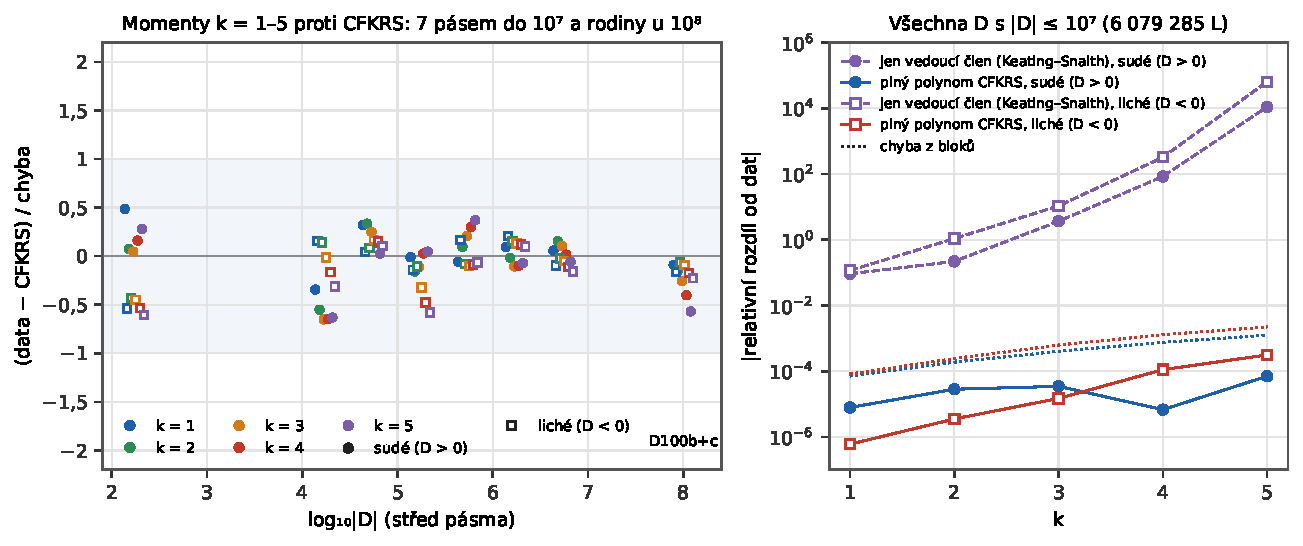
\includegraphics[width=1\textwidth,height=\textheight]{../../figures/01_moments_cz.pdf}
\caption{Obrázek 1. Vlevo: odchylka momentů \(k = 1\)--\(5\) od polynomů
CFKRS ve směrodatných chybách pro sedm pásem \(|D|\) do \(10^7\) a pro
rodiny u \(10^8\) (plné: sudé, prázdné: liché). Vpravo: relativní rozdíl
plného polynomu (plně) a samotného vedoucího členu (čárkovaně) od dat
přes všechna \(|D| \le 10^7\); tečkovaně chyba z bloků.}
\end{figure}

Členy nižšího řádu polynomu jsou podstatné: samotný vedoucí člen se mýlí
o 9 \% u \(k = 1\) a o faktor \(10^4\) u \(k = 5\). Rozdíl prvních
momentů obou znamének je čistý důsledek \(\Gamma\)-faktorů,
\(A_0(\psi(\tfrac34) - \psi(\tfrac14))/2 = A_0\pi/2 = 1{,}10654\); data
dávají \(1{,}10649 \pm 0{,}00060\).

\hypertarget{souvisluxe9-rodiny}{%
\subsection{4.2 Souvislé rodiny}\label{souvisluxe9-rodiny}}

Chyba z bloků je menší než chyba nezávislých hodnot, a to s faktory
0,11--0,33 pro \(k = 1\)--4 a 0,31--0,42 pro \(k = 5\), kdežto náhodné
podmnožiny stejné velikosti kolísají jako nezávislé hodnoty
(0,94--1,04). Součty \(L(\tfrac12, \chi_D)^k\) přes blok 20 000 po sobě
jdoucích \(|D|\) tedy kolísají třikrát až devětkrát méně než přes stejný
počet náhodných diskriminantů. Přes celý rozsah má kumulativní součet
reziduí střední kvadratickou velikost jen 0,008--0,028 náhodné procházky
nezávislých hodnot --- v souladu s pozorováním Aldersona a Rubinsteina,
že zbytek prvního momentu roste jen jako \(X^{1/4+\varepsilon}\)
{[}11{]}.

Jev roste se šířkou bloku \(w\) (obrázek 2 vlevo): pro \(k = 1\) a sudé
charaktery klesá poměr z 0,48 při \(w = 100\) na 0,27 při \(w = 10^3\),
0,15 při \(10^4\) a 0,062 při \(10^5\). U \(10^8\) ruší stejná šířka
méně (12 z 12 srovnání při \(w = 500\)--2 000). Mechanismem je
periodicita \(\chi_D(n)\) v \(D\): v přibližné funkcionální rovnici
přispívají členy s \(n\) zhruba do \(\sqrt{|D|}\), \(\chi_D(n)\) je v
\(D\) periodické s periodou \(n\) (nebo \(4n\)) a blok šířky \(w\)
průměruje členy s \(n \lesssim w\) přes celé periody. Vyrušení není
úplné, protože podmínka „fundamentální`` periodická není. Je to tentýž
jev souvislých rodin, který studie III našla v nízkofrekvenčním výkonu
nul.

\begin{figure}
\centering
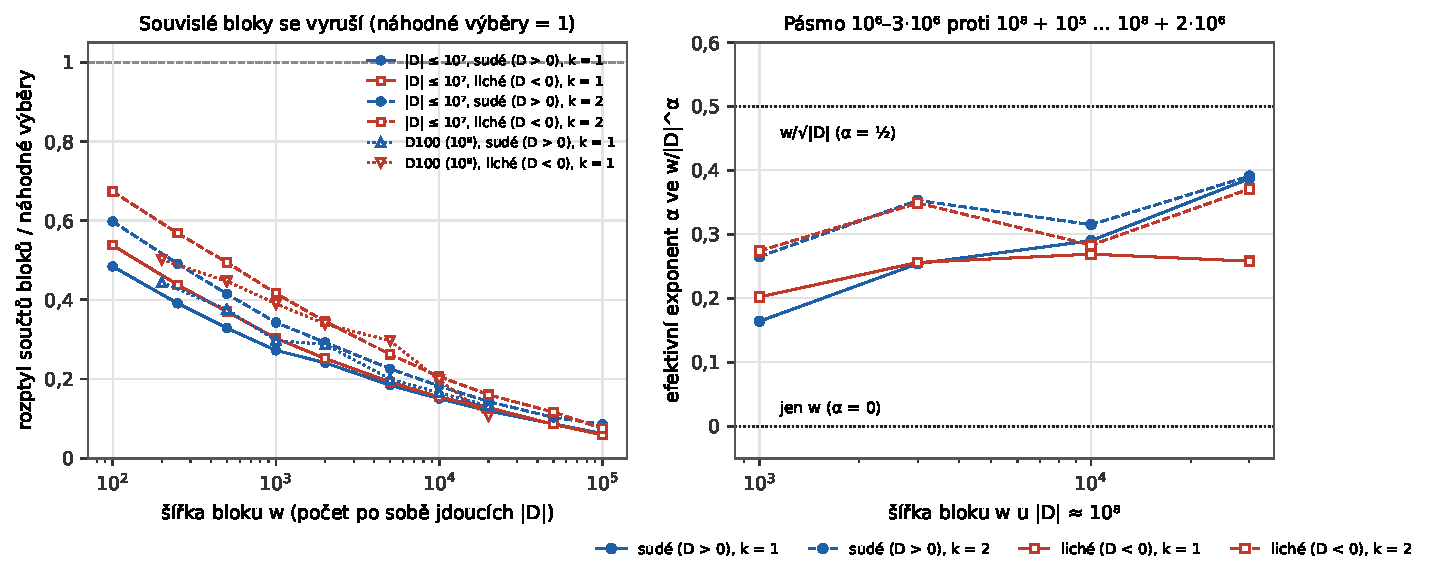
\includegraphics[width=1\textwidth,height=\textheight]{../../figures/02_blocks_cz.pdf}
\caption{Obrázek 2. Vlevo: rozptyl součtů přes bloky \(w\) po sobě
jdoucích \(|D|\) vůči náhodným výběrům stejné velikosti pro
\(|D| \le 10^7\) (\(k = 1, 2\)) a pro D100 u \(10^8\). Vpravo: efektivní
exponent \(\alpha\), při kterém se pásma u \(|D| \approx 2\cdot10^6\) a
\(10^8\) ruší stejně při stejném \(w/|D|^{\alpha}\).}
\end{figure}

Jak jev závisí na \(|D|\)? Dvě předem zapsaná pravidla byla zamítnuta.
Škálování s \(w/\sqrt{|D|}\) (délkou funkcionální rovnice) selhává až o
25 chyb: pásmo u \(2\cdot10^6\) ruší méně než pásmo u \(10^8\) se
stejným \(w/\sqrt{|D|}\); samotné \(w\) dává opačné znaménko (\(-2{,}9\)
až \(-13{,}7\) chyby) a \(w/|D|\) je daleko. Exponent \(\alpha\), který
obě pásma sladí, je 0,16--0,39 a roste s \(w\) (obrázek 2 vpravo).
Selhává i škálování s logaritmickou proměnnou
\(u = \ln w/\ln\sqrt{|D|}\) (14 z 16 srovnání se liší o víc než dvě
chyby, až o 15,9): pásma se shodnou pro
\(u_B \approx 0{,}87\)--\(0{,}99\,u_A\), což ukazuje na efektivní délku
funkcionální rovnice o něco větší než \(\sqrt{|D|}\). U \(10^8\) a
\(w = 10^5\) je poměr 0,09--0,14 (19 bloků). Kvantitativní zákon
vyrušení zůstává otevřený; pro momenty znamená, že chyba z bloků
souvislé rodiny je opatrná.

\hypertarget{rozdux11blenuxed-hodnot}{%
\subsection{4.3 Rozdělení hodnot}\label{rozdux11blenuxed-hodnot}}

\textbf{Hybridní model.} Rozptyl \(\ln L\) souhlasí s hybridem z oddílu
3.4 do 0,26 \% ve třech pásmech s \(|D| \ge 10^5\) (0,3--2,1 chyby;
chyba z bloků je 0,11--0,64 \%) pro obě znaménka, bez volného parametru.
Vyšší kumulanty se odchylují (obrázek 3 vlevo): pro \(|D| \ge 10^6\)
leží střední hodnota \(\ln L\) o 0,017--0,023 pod hybridem a třetí
kumulant je o 4--7 \% méně záporný (1,4--12,4 chyby; zamítnuto předem
zapsaným pravidlem). S \(2N = \ln(|D|/\pi)\) pro obě znaménka, jako v
původním modelu Keatinga a Snaithové, leží předpověď mezi znaménky.

\textbf{Zlomkové momenty.} \(E[L^{1/2}]\) a \(E[L^{-1/2}]\) pro
\(10^6 \le |D| \le 10^7\) leží asi 1 \% od hybridu
(\(-1{,}00;\ -0{,}76;\ -0{,}93;\ -0{,}73\) \% a
\(+0{,}94;\ +0{,}69;\ +0{,}88;\ +0{,}66\) \%, sudé/liché a dvě pásma);
pravidlo „do 1 \%`` bylo těsně nesplněno. Sledováno až do \(10^8\) klesá
odchylka monotonně ve všech čtyřech řadách (sudé, \(s = \tfrac12\):
\(-1{,}13\) \% při \(10^5\)--\(10^6\), \(-1{,}00\), \(-0{,}93\),
\(-0{,}80\) \% při \(10^8\)) a fit \(a + b/\ln|D|\) dává asymptoty
\(-0{,}09 \pm 0{,}23\), \(+0{,}10 \pm 0{,}38\), \(-0{,}26 \pm 0{,}21\) a
\(-0{,}03 \pm 0{,}43\) \% --- slučitelné s nulou, jak se čeká u členu
nižšího řádu (obrázek 3 vpravo). Předem zapsané pravidlo žádalo pokles o
víc než tři chyby mezi \(10^6\)--\(10^7\) a \(10^8\); dosáhl 0,5--2,4,
takže tvrzení je nerozhodnuté.

\begin{figure}
\centering
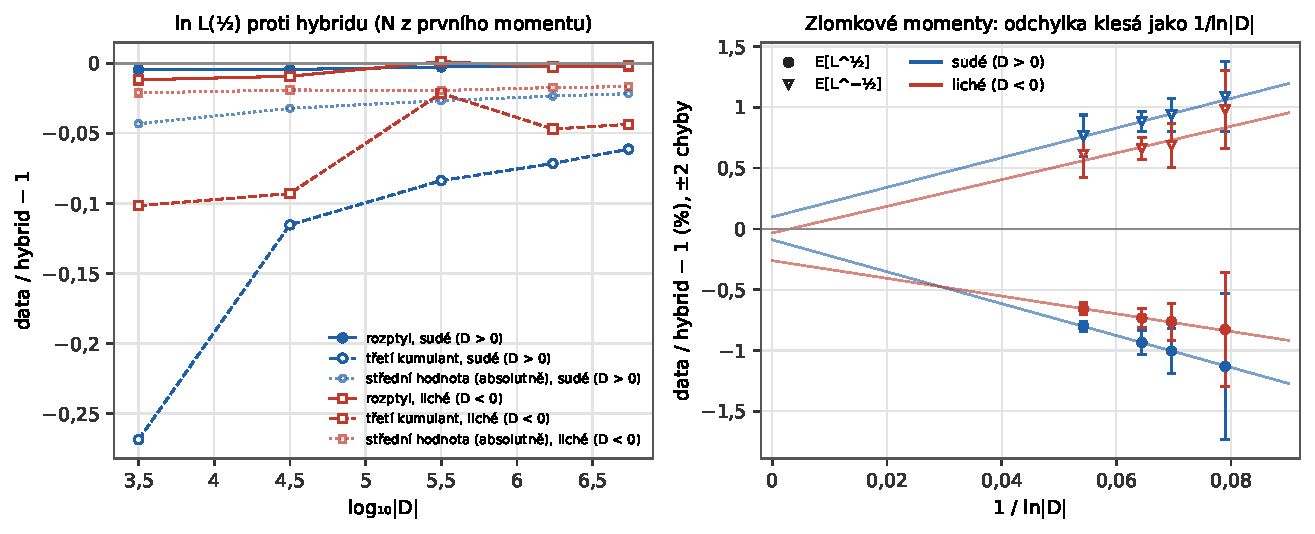
\includegraphics[width=1\textwidth,height=\textheight]{../../figures/03_log_values_cz.pdf}
\caption{Obrázek 3. Vlevo: střední hodnota, rozptyl a třetí kumulant
\(\ln L(\tfrac12)\) proti hybridnímu modelu po pásmech \(|D|\). Vpravo:
zlomkové momenty \(E[L^{\pm1/2}]\) proti hybridu v závislosti na
\(1/\ln|D|\) (\(\pm 2\) chyby) s lineárními fity; body vpravo jsou
nejmenší \(|D|\), vlevo \(10^8\).}
\end{figure}

\textbf{Malé hodnoty.} U náhodných matic má \(E[\Lambda^s]\) první pól v
\(s = -\tfrac32\), takže
\(P(\Lambda < \varepsilon) \propto \varepsilon^{3/2}\). Exponent hodnot
pod 0,03 odhadnutý maximální věrohodností je \(1{,}518 \pm 0{,}015\)
(\(1{,}525 \pm 0{,}022\) sudé, \(1{,}511 \pm 0{,}021\) liché; obrázek 4
vlevo). Hodnot pod \(\varepsilon\) je o 11--17 \% méně, než hybrid
předpovídá pro \(|D| \ge 10^6\) při \(\varepsilon = 0{,}1\) a 0,03
(obrázek 4 vpravo), stejně ve všech devíti třídách
\((\chi_D(2), \chi_D(3))\) (\(\chi^2 = 41{,}4\) při 32 stupních
volnosti, \(p = 0{,}12\)), ačkoli se třídy v počtu malých hodnot ohromně
liší (4 161 hodnot pod 0,03 pro \(\chi_D(2) = \chi_D(3) = -1\) proti 21
pro \(+1, +1\), obě znaménka, \(|D| \ge 10^6\)), jak jejich aritmetické
faktory předpovídají.

\begin{figure}
\centering
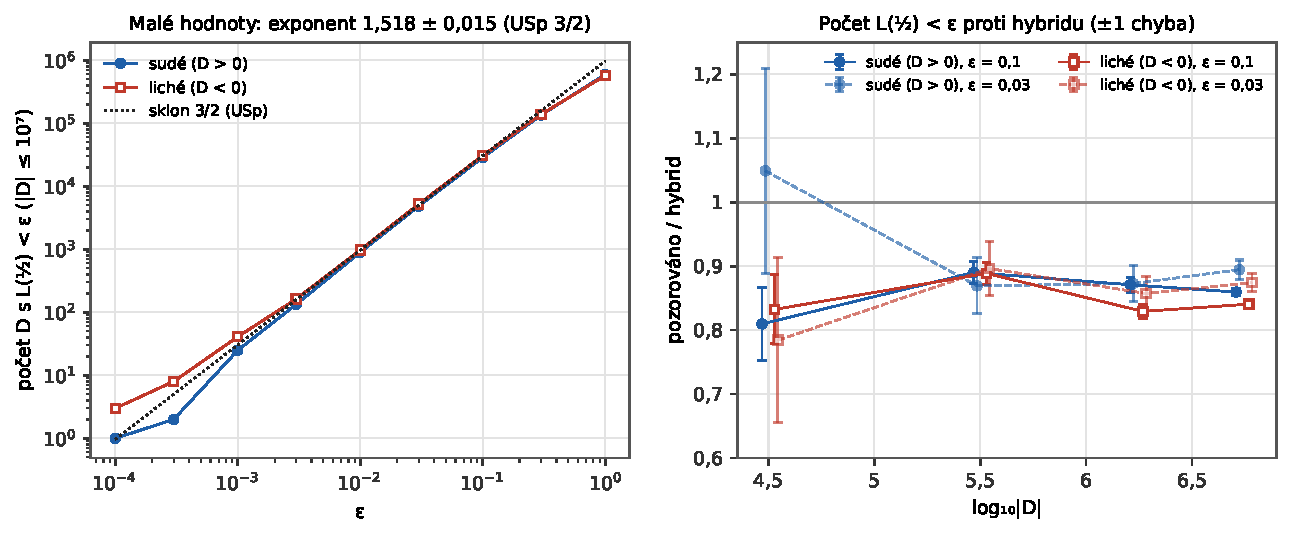
\includegraphics[width=1\textwidth,height=\textheight]{../../figures/04_small_values_cz.pdf}
\caption{Obrázek 4. Vlevo: počet diskriminantů s
\(L(\tfrac12) < \varepsilon\) pro \(|D| \le 10^7\) se sklonem
\(\tfrac32\) USp. Vpravo: pozorovaný počet proti hybridnímu modelu pro
\(\varepsilon = 0{,}1\) a 0,03 po pásmech \(|D|\).}
\end{figure}

\textbf{Nevymizení.} Žádná hodnota ve středu není nulová: nejmenší je
\(6{,}04\cdot10^{-5}\) u \(D = -115\,147\) (známý příklad; Watkins,
citovaný Stopplem {[}21{]}), 66 hodnot leží pod \(10^{-3}\). U \(10^8\)
a \(10^{10}\) jsou nejmenší hodnoty \(2{,}0\cdot10^{-4}\) a
\(2{,}8\cdot10^{-4}\).

\hypertarget{hodnota-ve-stux159edu-a-prvnuxed-nula}{%
\subsection{4.4 Hodnota ve středu a první
nula}\label{hodnota-ve-stux159edu-a-prvnuxed-nula}}

Hodnota ve středu a první nula \(x_1\) (rozvinutá pomocí \(\theta_D\)
jako ve studii III) jsou silně svázané:
\(\mathrm{corr}(\ln L, x_1) = 0{,}83\)--0,89 v osmi skupinách (čtyři
rodiny, dvě znaménka) a střední hodnota \(L\) roste z asi 0,7--1,0 v
nejnižší pětině \(x_1\) na 7,5--19 v nejvyšší. Promíchání dává
\(0{,}000 \pm 0{,}006\). USp\((2N_{k1})\) dává 0,81--0,89 a data leží
nad ním v sedmi z osmi skupin, až o 17 chyb (obrázek 5 vlevo); střední
první nula je níž než u USp\((2N_{k1})\) (0,62--0,69 proti 0,69--0,74).
Obě tvrzení byla zamítnuta; nadbytek nenesou malá prvočísla --- uvnitř
tříd \(\chi_D(2), \chi_D(3), \chi_D(5)\) se vzdálenost od USp spíš
zvětší, než zmenší.

S \(N_{\mathrm{ef}}\) z domněnky poměrů (bez volného parametru) se obraz
mění: \(N_{\mathrm{ef}}\) se téměř přesně rovná velikosti \(N_{x_1}\),
která sedí se střední první nulou (1,98 proti 2,00 u B10 sudých, \ldots,
3,88 proti 3,88 u D100 lichých), takže střední první nula je jev konečné
velikosti, který domněnka poměrů vysvětlí (do 3,2 chyby kromě C100
sudých, 6,9). Zbývá posun první nuly při vážení hodnotou
\(L(\tfrac12)\): v datech je o 9--16 \% větší než u
USp\((2N_{\mathrm{ef}})\) váženého \(\Lambda(1)\) (8--42 chyb; obrázek 5
vpravo). Nadbytek vazby hodnoty a nuly tedy není jevem konečné velikosti
matice; vážená hustota domněnky poměrů ho popisuje pro obě znaménka
(oddíl 4.6).

\begin{figure}
\centering
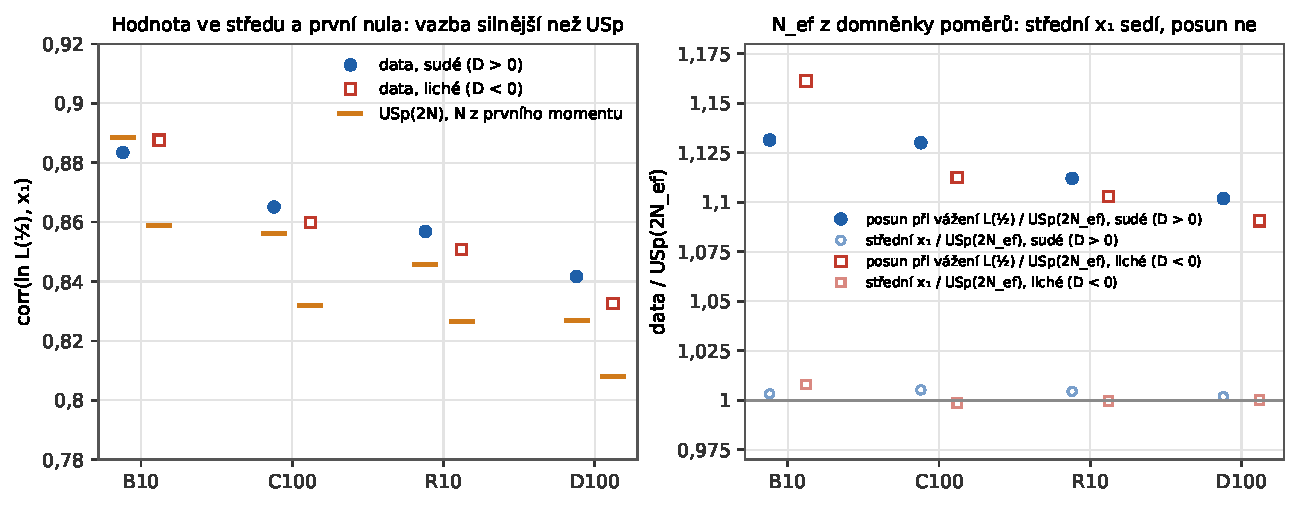
\includegraphics[width=1\textwidth,height=\textheight]{../../figures/05_first_zero_cz.pdf}
\caption{Obrázek 5. Vlevo: korelace \(\ln L(\tfrac12)\) s první nulou ve
čtyřech rodinách proti USp\((2N)\) s \(N\) z prvního momentu. Vpravo:
posun střední první nuly při vážení \(L(\tfrac12)\) a samotná střední
první nula, obojí vůči USp\((2N_{\mathrm{ef}})\) s \(N_{\mathrm{ef}}\) z
domněnky poměrů.}
\end{figure}

Malé hodnoty a nízké nuly chodí spolu, jak předpovídají náhodné matice.
Hough {[}12{]} ukázal, že logaritmus \(L(\tfrac12, \chi_{8d})\) je
Gaussův, pokud jsou nízké nuly vzácné; v našich datech je
\(P(L < 0{,}03 \mid x_1 < 0{,}2)/P(L < 0{,}03) = 27\)--44 v osmi
skupinách a USp\((2N_{x_1})\) se shodnými kvantily dává 32--42 (nejvýš
1,0 chyby; promíchané hodnoty dávají 1).

\hypertarget{hybridnuxed-souux10diny-a-ux10dlen-x34}{%
\subsection{\texorpdfstring{4.5 Hybridní součiny a člen
\(X^{3/4}\)}{4.5 Hybridní součiny a člen X\^{}\{3/4\}}}\label{hybridnuxed-souux10diny-a-ux10dlen-x34}}

\textbf{Domněnka o rozdělení momentů.} Gonek, Hughes a Keating {[}13{]}
a Bui a Keating {[}14{]} zapisují \(L\) jako součin \(P_X Z_X\) krátkého
Eulerova součinu a součinu přes nuly a vyslovují domněnku, že se momenty
asymptoticky rozdělí, \(E[L^k] \approx E[P_X^k]E[Z_X^k]\). S useknutým
Eulerovým součinem je poměr \(S_k = E[L^k]/(E[P_X^k]E[Z_X^k])\) daleko
od 1 (\(S_1 = 0{,}80\) při \(X = 10\); zamítnuto). S \(P_X\) ve tvaru
Buie a Keatinga (\(\exp\sum_{n \le X}\Lambda(n)\chi(n)/(\sqrt n\ln n)\))
se \(S_k\) s vodičem blíží 1 ve všech čtyřech řadách (podpořeno):
\(S_1\) pro sudé charaktery 0,863 (\(10^5\)--\(10^6\)), 0,897
(\(3\cdot10^6\)--\(10^7\)), 0,926 (\(10^8\)), pro liché 0,904, 0,928,
0,949; \(S_2\) 0,50 → 0,58 → 0,65 a 0,59 → 0,66 → 0,72. Momenty \(Z_X\)
proti USp\((2N)\) s \(N = \ln|D|/(2e^\gamma\ln X)\) (1,5--3,2) sedí pro
liché charaktery u \(k = 1\) (poměr 0,94--1,10), ale ne pro sudé
(0,49--0,96); tvrzení bylo zamítnuto. (Předem zapsané pravidlo vzalo
\(N = \ln|D|/(e^\gamma\ln X)\), což je v {[}14{]} velikost matice
\(2N\); se správným \(N\) závěr zůstává.)

\textbf{Člen \(X^{3/4}\).} Pro \(k = 3\) dává běžný součet reziduí
dělený \(X^{3/4}\) pro sudé charaktery \(b = -0{,}248 \pm 0{,}038\) ---
6,6 chyby od nuly a 2,9 od hodnoty \(b_+ \approx -0{,}14\), kterou
spočetl Zhang a cituje {[}11{]} --- a pro liché
\(-0{,}219 \pm 0{,}130\), nerozlišeno. V podrodině \(D = 8d\) Diaconua a
Whiteheada {[}10{]} s jejich vyhlazením je signál \(-28\) proti rozptylu
asi 200 mezi okny a \(b = -0{,}26 \pm 0{,}21\); obě tvrzení jsou
nerozhodnutá. Polynom CFKRS podrodiny (s faktorem u 2) souhlasí s
vyhlazeným součtem do \(5\cdot10^{-5}\) a sousední okna opět kolísají
31krát méně než nezávislá.

\hypertarget{vuxe1ux17eenuxe1-hustota-nuxedzkuxfdch-nul}{%
\subsection{4.6 Vážená hustota nízkých
nul}\label{vuxe1ux17eenuxe1-hustota-nuxedzkuxfdch-nul}}

Vážení nul hodnotou \(L(\tfrac12, \chi_D)\) je odtlačuje od středu.
Čistá USp\((2N_{x_1})\) selhává ve všech rodinách (\(\chi^2\) = 82--1
811 na pěti koších). Domněnka poměrů s vahou \(L(\tfrac12)\) (Fazzari
{[}17{]}) popisuje obě znaménka ve všech rodinách (obrázek 6): s větší z
obou chyb je \(\chi^2\) na pěti koších 0,63, 1,76, 0,87 a 4,31 pro sudé
charaktery v B10, C100, R10 a D100 a 0,52--1,26 pro liché; u \(10^8\)
(D100 ∪ D100b ∪ D100c, 1 215 839 L-funkcí) 2,25 a 0,72, u \(10^{10}\)
(E, 121 557 L-funkcí) 1,51 a 0,88; v rodinách spočtených až po opravě
(níže) 0,21 a 0,64 (S7) a 1,75 a 1,31 (S9L u \(10^9\)); nejmenší \(p\) z
dvaceti skupin je 0,51. Všechna tato \(\chi^2\) leží pod počtem košů
(průměr 1,3): chyba je opatrná, protože bereme větší ze dvou odhadů a
protože průměry přes souvislé rodiny kolísají méně než přes náhodné
výběry (oddíl 4.2). V popisné zkoušce na 20 kusech S7 je průměrné
\(\chi^2\) kusu 1,2 (sudé) a 1,9 (liché) u po sobě jdoucích kusů a 3,2 a
2,4 u náhodných; se samotnou chybou z bootstrapu 2,0 a 4,2 proti 6,1 a
5,1, kde se čeká 5. Test je tedy konzervativní a jeho hodnoty \(p\) jsou
jen orientační; že přesto rozlišuje, ukazuje chybná předpověď
(\(\chi^2\) až 285, níže). Promíchané hodnoty dávají nulu a nevážená
hustota i \(\langle L(\tfrac12)\rangle\) z téhož receptu souhlasí s daty
u obou znamének.

\begin{figure}
\centering
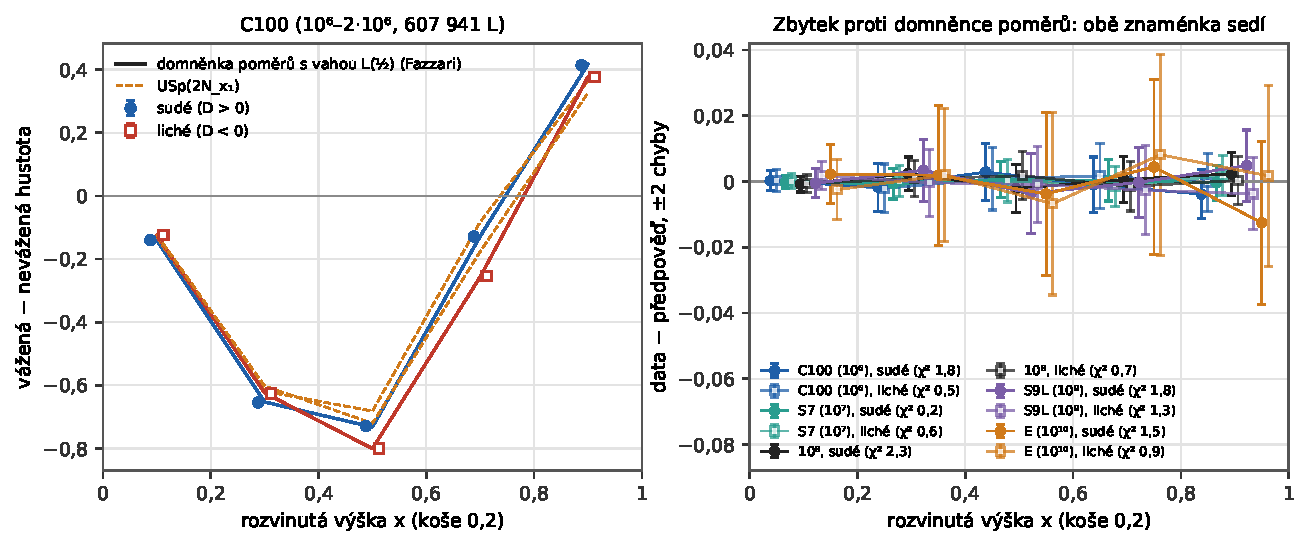
\includegraphics[width=1\textwidth,height=\textheight]{../../figures/06_weighted_density_cz.pdf}
\caption{Obrázek 6. Vlevo: vážená minus nevážená hustota nízkých nul v
C100 proti domněnce poměrů s vahou \(L(\tfrac12)\) (plně) a
USp\((2N_{x_1})\) (čárkovaně). Vpravo: data minus předpověď pro C100,
pro S7 a S9L (obě spočtené po opravě), pro 1,2 milionu L-funkcí u
\(10^8\) a pro E u \(10^{10}\); obě znaménka s předpovědí souhlasí.}
\end{figure}

\textbf{Oprava před vydáním.} Naše první implementace této předpovědi
(kroky laboratoře 34.79--34.84) obsahovala chybu: ve členu receptu s
oběma výměnami \(\alpha \to -\alpha\), \(\beta \to -\beta\) použila
faktor \(X(\tfrac12 + \alpha + \beta)\) místo
\(X(\tfrac12 + \alpha)X(\tfrac12 + \beta)\). Chyba mění předpověď pro
liché charaktery jen málo (nejvýš o 0,5 chyby dat), pro sudé silně, a s
vodičem slábne. S ní se zdálo, že sudá data nesou člen navíc (\(\chi^2\)
= 202 v B10 a 285 v C100), jehož amplituda klesala zhruba jako
\(|D|^{-1/4}\); zákon škálování i replikace na nových diskriminantech u
\(10^8\) byly zapsány předem a prošly --- testovaly ovšem chybu
předpovědi, ne vlastnost nul. Druhá implementace, psaná z první pro
třídy \(\chi_D(2)\), chybu sdílela, a proto se obě shodovaly. Před
vydáním jsme podle pravidla zapsaného předem napsali nezávislou
implementaci: lokální faktory jako numericky sčítané řady místo
uzavřených tvarů, Eulerův součin do \(5\cdot10^5\), derivaci podle
\(\beta\) centrální diferencí a limitu \(\alpha \to 0\) Richardsonovou
extrapolací. Od první se lišila až o 13,3 chyby u sudých charakterů, což
vedlo k chybnému faktoru; po opravě tohoto jediného faktoru se první
implementace shoduje s nezávislou na 0,005 chyby (absolutně
\(3\cdot10^{-5}\)). Obrázek 7 ukazuje zdánlivý člen a jeho zmizení: na
tvaru dřívější odchylky jsou amplitudy sudých nyní
\(0{,}065 \pm 0{,}059\) (C100), \(-0{,}038 \pm 0{,}050\) (všechny tři
rodiny u \(10^8\)) a \(0{,}08 \pm 0{,}19\) (E), všechny nulové v rámci
chyb.

\begin{figure}
\centering
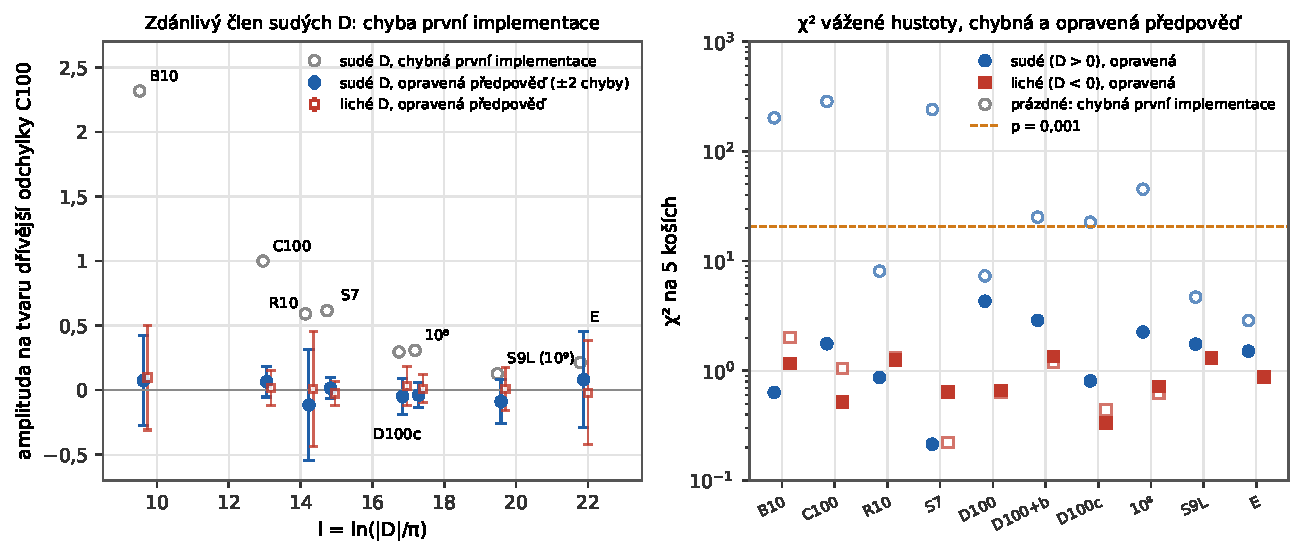
\includegraphics[width=1\textwidth,height=\textheight]{../../figures/07_correction_cz.pdf}
\caption{Obrázek 7. Vlevo: amplituda na tvaru dřívější odchylky C100
proti \(l = \ln(|D|/\pi)\) s chybnou první implementací (prázdně) a s
opravenou předpovědí (plně, \(\pm 2\) chyby; liché charaktery
čtverečky). Vpravo: \(\chi^2\) na pěti koších ve všech skupinách s
chybnou (prázdně) a opravenou předpovědí (plně); čárkovaně
\(p = 0{,}001\).}
\end{figure}

\textbf{Rodina spočtená po opravě.} Jakmile byla chyba nalezena, zapsali
jsme před jakýmikoli novými daty ještě jedno pravidlo: opravená
předpověď musí pro obě znaménka a s \(p > 0{,}001\) na pěti koších
popsat rodinu, která dosud nebyla vyhodnocena. Počítač 2 pak spočetl
nuly všech fundamentálních diskriminantů s
\(7{,}5\cdot10^6 < |D| \le 10^7\) (S7: 1 519 830 L-funkcí, 6 592 004
nul; 16 860 z těchto diskriminantů patří i do náhodného výběru R10).
Opravená předpověď dává \(\chi^2 = 0{,}21\) pro sudé a \(0{,}64\) pro
liché charaktery (\(p = 0{,}999\) a \(0{,}986\)) a amplituda na tvaru
dřívější odchylky je \(0{,}015 \pm 0{,}040\). Chybná první implementace
by u sudých charakterů dala \(\chi^2 = 240{,}7\) a amplitudu \(0{,}62\)
--- právě to, co pro tuto rodinu předpověděl zákon škálování s ní
proložený (\(0{,}608 \pm 0{,}045\), zapsáno dřív, než byla chyba známa).
Předpověď zapsaná předem tedy chrání před pružným vyhodnocením, ne před
chybou společnou předpovědi i vyhodnocení; s opravenou předpovědí leží
amplituda 9,8 chyby pod tímto očekáváním.

\textbf{Bod u \(10^9\).} Aby se vyplnila mezera mezi \(10^8\) a
\(10^{10}\), spočetl pak počítač 2 podle téhož pravidla (zapsaného před
daty spolu s ostatními rozhodnutími pro tuto rodinu) nuly všech
fundamentálních diskriminantů s \(10^9 < |D| \le 10^9 + 8\cdot10^5\)
(S9L: 486 344 L-funkcí, 2 099 543 nul, 19,7 hodiny); hodnoty ve středu
pocházejí z naší funkcionální rovnice a k vyhodnocení byly uvolněny až
poté, co prošla kontrola proti PARI z oddílu 2. Opravená předpověď dává
\(\chi^2 = 1{,}75\) pro sudé a \(1{,}31\) pro liché charaktery
(\(p = 0{,}883\) a \(0{,}934\)) a amplituda na tvaru dřívější odchylky
je \(-0{,}088 \pm 0{,}084\). Chybná první implementace by u sudých
charakterů dala \(\chi^2 = 4{,}7\) a amplitudu \(0{,}13\); obě amplitudy
se liší o 2,6 chyby. Pro tento bod byla zapsána hypotéza dřív, než byla
chyba známa (amplituda \(0{,}164 \pm 0{,}040\) čekaná ze zákona
škálování proloženého s chybnou předpovědí); s opravenou předpovědí její
pravidlo při dosažené chybě tuto hodnotu od nuly neoddělí (leží od sebe
méně než dvě složené chyby). Naměřená amplituda leží 2,7 složené chyby
pod čekanou hodnotou; formální výsledek pravidla (NEROZHODNUTO) uvádíme
jen pro záznam a nevykládáme jej. Explicitní vzorec jsme na S9L
nevyhodnocovali: jeho strana prvočísel by sahala do
\(n \le |D|/\pi \approx 3{,}2\cdot10^8\) (rozhodnuto předem).

\textbf{Explicitní vzorec.} Jako kontrolu, která domněnku poměrů
nepoužívá, jsme na C100 vyhodnotili explicitní vzorec s testovací funkcí
\(\varphi(u) = (\sin(\pi u/2)/(\pi u/2))^4\),
\(u = \gamma\ln(|D|/\pi)/2\pi\), jejíž Fourierova transformace má nosič
\(|\nu| \le 1\), takže strana prvočísel končí u \(n \le |D|/\pi\)
(konvence jsme ověřili na jednotlivých L-funkcích s nulami z PARI do
\(u = 40\), na \(10^{-6}\)). Na každé L-funkci se strana nul (nuly
studie III, část nad spočtenými nulami z hladké hustoty) a strana
prvočísel (charaktery, \(\Lambda(n)\) a \(\Gamma\)-člen) shodují s
mediánem \(7\cdot10^{-5}\). Pro rozdíl vážených a nevážených průměrů
rodiny je strana nul \(-0{,}36855 \pm 0{,}00073\) (sudé) a
\(-0{,}45488 \pm 0{,}00096\) (liché); s částí nad spočtenými nulami z
hustot domněnky poměrů, jak předepisovalo pravidlo zapsané předem, se
strana nul a strana prvočísel shodují na 2,2 a 1,6 párové chyby (se
samotnou hladkou hustotou na 5,1 a 9,0, rozdíl \(2\cdot10^{-5}\)).
Strana prvočísel se dělí (obrázek 8) na \(p = 2\) (\(-0{,}091\) /
\(-0{,}095\)), lichá \(p \le \sqrt{|D|/\pi}\) (\(-0{,}271\) /
\(-0{,}331\)), lichá \(p > \sqrt{|D|/\pi}\) (\(+0{,}019\) /
\(-0{,}002\)) a mocniny prvočísel (\(-0{,}025\) / \(-0{,}027\)). Se
stejnou hladkou testovací funkcí se opravená předpověď liší od strany
nul o \(-0{,}09\) a \(-0{,}04\) chyby. Na S7 (759 933 + 759 897
L-funkcí) je strana nul \(-0{,}38687 \pm 0{,}00052\) (sudé) a
\(-0{,}46553 \pm 0{,}00060\) (liché), strana nul a strana prvočísel se
shodují na 2,0 a 0,1 párové chyby a opravená předpověď se od strany nul
liší o \(-0{,}12\) a \(-0{,}12\) chyby. Párová chyba je tu jen
\(4{,}4\cdot10^{-7}\) a \(1{,}3\cdot10^{-6}\), takže na části nad
spočtenými nulami záleží: explicitní vzorec pro ni žádá
\(2{,}35\cdot10^{-5}\) a \(3{,}13\cdot10^{-5}\) a hustoty domněnky
poměrů dávají \(2{,}26\cdot10^{-5}\) a \(3{,}14\cdot10^{-5}\).

\begin{figure}
\centering
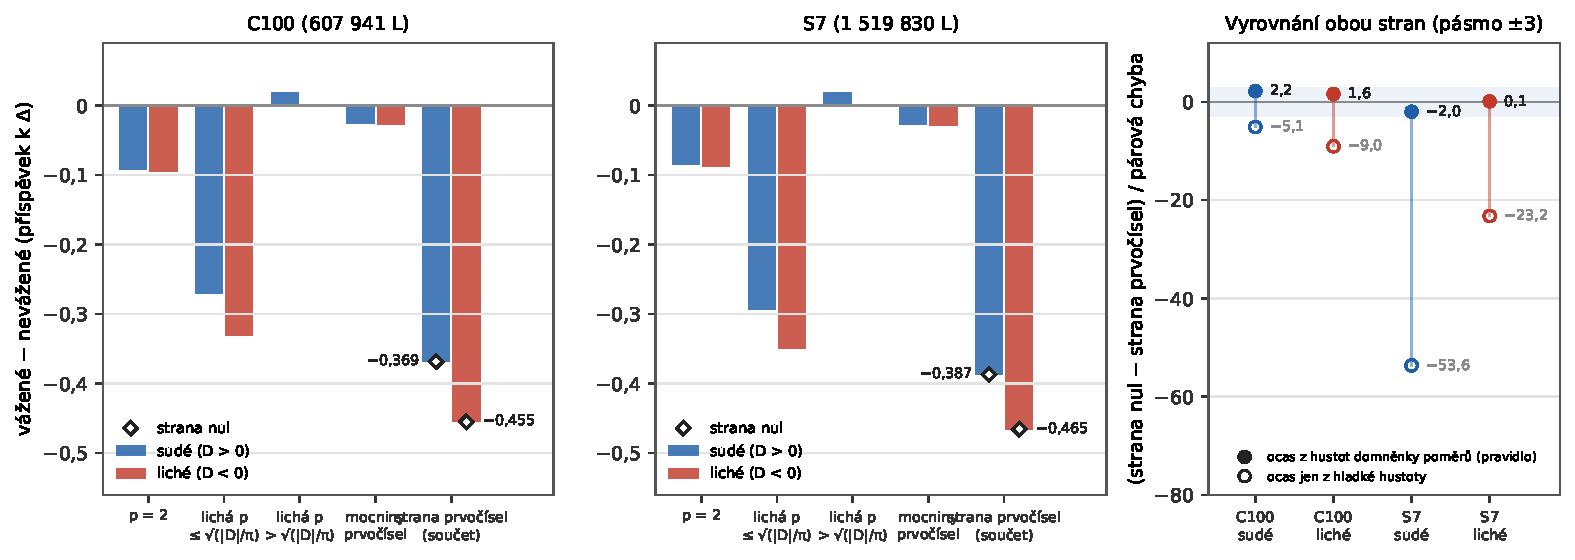
\includegraphics[width=1\textwidth,height=\textheight]{../../figures/08_explicit_formula_cz.pdf}
\caption{Obrázek 8. Explicitní vzorec pro rozdíl vážených a nevážených
průměrů rodiny. Vlevo a uprostřed: části strany prvočísel (sloupce;
\(\Gamma\)-člen řádu \(10^{-5}\) není vidět), jejich součet a strana nul
(kosočtverce) na C100 a S7. Vpravo: strana nul minus strana prvočísel v
jednotkách párové chyby, s částí nad spočtenými nulami jen z hladké
hustoty (prázdně) a z hustot domněnky poměrů, jak předepisovalo pravidlo
(plně); pásmo: \(\pm 3\) chyby.}
\end{figure}

\hypertarget{tvrzenuxed-a-jejich-stav}{%
\section{5. Tvrzení a jejich stav}\label{tvrzenuxed-a-jejich-stav}}

{\small\begin{longtable}[]{@{}
  >{\raggedright\arraybackslash}p{(\columnwidth - 2\tabcolsep) * \real{0.5435}}
  >{\raggedright\arraybackslash}p{(\columnwidth - 2\tabcolsep) * \real{0.4565}}@{}}
\toprule\noalign{}
\begin{minipage}[b]{\linewidth}\raggedright
tvrzení
\end{minipage} & \begin{minipage}[b]{\linewidth}\raggedright
stav
\end{minipage} \\
\midrule\noalign{}
\endhead
\bottomrule\noalign{}
\endlastfoot
Momenty \(k = 1\)--\(4\) obou znamének se řídí plnými polynomy CFKRS
{[}5{]} do \(10^7\). & Známá domněnka, dříve testovaná do
\(|d| \approx 5\cdot10^{10}\) {[}11{]}; zde v souladu v 56 pásmech i
výběrech (pravidlo: PODPOŘENO). \\ \addlinespace[2pt]
Pátý moment se řídí CFKRS. & V souladu: 14 pásem, \(\le 0{,}63\) chyby
(PODPOŘENO). \\ \addlinespace[2pt]
Momenty se řídí CFKRS u \(10^8\) (\(k = 1\)--5). & V souladu:
\(\le 0{,}57\) chyby (PODPOŘENO). \\ \addlinespace[2pt]
Samotný vedoucí člen Keatinga a Snaithové popisuje momenty do 10 \%. &
Zamítnuto: 9 \% u \(k = 1\) až faktor \(6\cdot10^4\) u \(k = 5\). \\ \addlinespace[2pt]
Rozdíl prvních momentů lichých a sudých charakterů je \(A_0\pi/2\). & V
souladu: \(1{,}10649 \pm 0{,}00060\) proti 1,10654 (PODPOŘENO). \\ \addlinespace[2pt]
Součty přes bloky po sobě jdoucích diskriminantů kolísají jako náhodné
výběry. & Zamítnuto: 0,11--0,42 náhodných výběrů. \\ \addlinespace[2pt]
Vyrušení roste se šířkou bloku a je slabší při větším \(|D|\). & V
souladu (PODPOŘENO; dodatečně). \\ \addlinespace[2pt]
Vyrušení závisí na \(|D|\) jen přes \(w/\sqrt{|D|}\), nebo přes
\(\ln w/\ln\sqrt{|D|}\). & Zamítnuto: až 25 a 15,9 chyby; efektivní
exponent 0,16--0,39. \\ \addlinespace[2pt]
Rozptyl \(\ln L\) se řídí hybridním modelem do 1 \%. & V souladu: 0,26
\% (PODPOŘENO). \\ \addlinespace[2pt]
Třetí kumulant a zlomkové momenty \(E[L^{\pm1/2}]\) se řídí hybridem. &
Zamítnuto: 4--7 \% a asi 1 \%. \\ \addlinespace[2pt]
Odchylka zlomkových momentů klesá jako \(1/\ln|D|\) k nule. &
Nerozhodnuto: klesá monotonně do \(10^8\), asymptota v rámci chyb 0,
pokles 0,5--2,4 chyby (pravidlo: 3). \\ \addlinespace[2pt]
\(P(L < \varepsilon) \propto \varepsilon^{3/2}\). & V souladu:
\(1{,}518 \pm 0{,}015\) (PODPOŘENO; dodatečně). \\ \addlinespace[2pt]
Schodek malých hodnot proti hybridu je stejný ve všech třídách
\(\chi_D(2)\), \(\chi_D(3)\). & V souladu: \(p = 0{,}12\)
(PODPOŘENO). \\ \addlinespace[2pt]
Žádné \(L(\tfrac12, \chi_D)\) nevymizí pro \(|D| \le 10^7\). & V
souladu: nejmenší \(6{,}04\cdot10^{-5}\) (PODPOŘENO). \\ \addlinespace[2pt]
Korelace \(\ln L\) s první nulou a střední první nula se řídí
USp\((2N_{k1})\). & Zamítnuto: až 17,7 a 42 chyb. \\ \addlinespace[2pt]
Nadbytek korelace nesou malá prvočísla. & Zamítnuto. \\ \addlinespace[2pt]
\(N_{\mathrm{ef}}\) z domněnky poměrů vysvětlí první nulu i její posun
při vážení \(L(\tfrac12)\). & Zčásti: střední první nulu ano, posun ne
(o 9--16 \% výš; ZAMÍTNUTO). \\ \addlinespace[2pt]
Malé hodnoty a nízké nuly chodí spolu jako v USp\((2N_{x_1})\). & V
souladu: poměr 27--44 proti 32--42 (PODPOŘENO). \\ \addlinespace[2pt]
Momenty se rozdělí na \(P_X\) a \(Z_X\) (Bui--Keating). & V souladu s
pomalým přiblížením k 1 (PODPOŘENO); useknutý součin zamítnut. \\ \addlinespace[2pt]
Momenty \(Z_X\) se řídí USp\((2N)\) s \(N = \ln|D|/(2e^\gamma\ln X)\). &
Zamítnuto pro sudé charaktery (0,49--0,96). \\ \addlinespace[2pt]
Člen \(bX^{3/4}\) je ve třetím momentu do \(10^7\) vidět. &
Nerozhodnuto: sudé \(-0{,}248 \pm 0{,}038\), liché nerozlišeno;
podrodina \(8d\): \(-0{,}26 \pm 0{,}21\). \\ \addlinespace[2pt]
Vážená hustota nízkých nul se řídí domněnkou poměrů s vahou
\(L(\tfrac12)\) {[}17{]}. & V souladu pro obě znaménka při všech
vodičích, \(\chi^2\) 0,2--4,3 na pěti koších (PODPOŘENO po opravě z
oddílu 4.6; s chybnou první implementací byly sudé charaktery do
\(10^8\) zamítnuty). \\ \addlinespace[2pt]
Opravená předpověď popíše rodinu spočtenou až po opravě (S7; pravidlo
zapsané před jejími daty). & V souladu: \(\chi^2\) 0,21 a 0,64, \(p\)
0,999 a 0,986 (PODPOŘENO). \\ \addlinespace[2pt]
Opravená předpověď popíše rodinu u \(10^9\) spočtenou až po opravě (S9L;
pravidlo zapsané před jejími daty). & V souladu: \(\chi^2\) 1,75 a 1,31,
\(p\) 0,883 a 0,934 (PODPOŘENO). \\ \addlinespace[2pt]
Nezávislá implementace zopakuje naši první implementaci předpovědi. &
Zamítnuto: až 13,3 chyby u sudých charakterů; chybný \(\Gamma\)-faktor
nalezen a opraven, pak shoda na 0,005 chyby. \\ \addlinespace[2pt]
Sudé charaktery nesou ve vážené hustotě člen navíc, který klesá jako
\(|D|^{-\theta}\) a zopakuje se u \(10^8\). & Po opravě zamítnuto:
amplitudy nulové v rámci chyb při každém vodiči (dřívější verdikty
PODPOŘENO stály na chybné předpovědi). \\ \addlinespace[2pt]
Explicitní vzorec vyrovná stranu nul a stranu prvočísel vážených průměrů
rodiny. & V souladu na C100 (2,2 a 1,6 chyby) i na S7 (2,0 a 0,1 chyby)
(PODPOŘENO). \\ \addlinespace[2pt]
\end{longtable}}

\hypertarget{co-je-novuxe9-a-co-potvrzenuxe9}{%
\section{6. Co je nové a co
potvrzené}\label{co-je-novuxe9-a-co-potvrzenuxe9}}

\textbf{Potvrzeno.} Polynomy CFKRS pro \(k = 1\)--5 a obě znaménka,
uzavřený tvar \(Q_1\) a vedoucí koeficienty Keatinga a Snaithové;
exponent \(\tfrac32\) malých hodnot; nevymizení ve spočteném rozsahu;
popis obou znamének váženou hustotou domněnky poměrů {[}17{]} od
\(10^4\) do \(10^{10}\); pomalé přibližování domněnky Buie a Keatinga o
rozdělení momentů {[}14{]}.

\textbf{Nové, pokud jsme mohli zjistit} (prohledali jsme arXiv, časopisy
a citace {[}11{]}, {[}14{]} a {[}17{]} ve dnech 8.--13. listopadu 2026):
jev souvislých rodin u momentů hodnot ve středu, jeho závislost na šířce
bloku a na \(|D|\) se zamítnutím škálování \(w/\sqrt{|D|}\) a
\(\ln w/\ln\sqrt{|D|}\); srovnání zlomkových momentů, třetího kumulantu
a malých hodnot s hybridním modelem bez volného parametru s odchylkami
klesajícími k \(10^8\); společná statistika hodnoty ve středu a první
nuly na 783 443 L-funkcích ve čtyřech rodinách (počítáno po rodinách;
R10 sdílí 6 740 diskriminantů s C100), kde \(N_{\mathrm{ef}}\) vysvětlí
střední první nulu, ale ne její posun při vážení; a kontrola vážené
hustoty explicitním vzorcem na 607 941 a 1 519 830 L-funkcích (C100 a
S7) se stranou prvočísel spočtenou z naměřených hodnot ve středu.

\hypertarget{omezenuxed}{%
\section{7. Omezení}\label{omezenuxed}}

\textbf{Věta, domněnka, pozorování.} Momenty \(k \le 3\) jsou věty (pro
\(k = 3\) v podrodině), polynomy CFKRS, hybridní modely a domněnka
poměrů jsou domněnky a vše, co zde měříme, je numerické pozorování při
konečném vodiči. Shoda domněnku podporuje, nedokazuje ji, a nic zde se
netýká zobecněné Riemannovy hypotézy.

\textbf{Rozsah.} Všechny diskriminanty do \(10^7\) leží hluboko pod
rozsahem Aldersona a Rubinsteina {[}11{]}; u \(10^8\), \(10^9\) a
\(10^{10}\) máme úplné úseky, ne úplné rozsahy. Nuly sahají do rozvinuté
výšky 4,3 a vstupují jen přes první nulu a hustotu na \([0, 1]\).

\textbf{Statistika.} Chyba z bloků je pro souvislé rodiny opatrná (oddíl
4.2), takže \(z\)-hodnoty momentů jsou menší než skutečné. Pravidla
kroku 34.76 byla zapsána po prvním pohledu na data a čtyři hypotézy jsou
dodatečné. Srovnání s USp závisí na volbě \(N\); používáme tři volby
určené bez volného parametru a uvádíme všechny.

\textbf{Předpověď vážené hustoty.} Naše první implementace měla chybu v
jednom faktoru a ta přežila druhou implementaci odvozenou z první, zákon
škálování i replikaci zapsanou předem; našla ji až nezávislá
implementace (oddíl 4.6). Opravená předpověď nyní souhlasí se dvěma
implementacemi, které nesdílejí kód, s explicitním vzorcem i se dvěma
rodinami spočtenými dodatečně podle pravidel zapsaných před jejich daty,
ale domněnka poměrů zůstává domněnkou a data ji testují jen pěti koši na
\([0, 1]\) a jednou hladkou testovací funkcí s nosičem do 1.

\hypertarget{vuxfdhled}{%
\section{8. Výhled}\label{vuxfdhled}}

Dalšími kroky jsou: váha \(L(\tfrac12)^2\) (Fazzariho rov. (4.10)) s
oběma implementacemi; a zákon vyrušení souvislých rodin. Samostatný směr
práce, který není součástí této studie, zkoumá fázové singularity
okénkových exponenciálních součtů přes nuly \(\zeta(s)\) při
iracionálním úhlu rotace, v rámci teorie vlnových dislokací a fázových
vírů {[}22--25{]} a renormalizace curlicues {[}26{]}; průzkumná poznámka
je k dispozici {[}27{]}.

\hypertarget{reprodukovatelnost}{%
\section{9. Reprodukovatelnost}\label{reprodukovatelnost}}

Repozitář (GitHub, archivovaný na Zenodu) obsahuje hodnoty ve středu pro
všechny diskriminanty tabulky 1 (\texttt{data/central\_values/}, soubory
NumPy s \(D\) a \(L(\tfrac12, \chi_D)\), rozdělené na části pod 20 MB,
se SHA-256), polynomy CFKRS, všechna čísla tohoto článku v jednom
souboru (\texttt{data/results/study\_v\_results.json}), pravidla zapsaná
předem (\texttt{data/rules/}, česky, s daty), manifesty a SHA-256 všech
bloků hodnot a nul a kód: \texttt{code/figures\_v.py} kreslí obrázky ze
souboru výsledků, \texttt{code/independent\_check\_v.py} přepočítá
hlavní čísla z hodnot ve středu kódem, který nesdílí nic se skripty,
které je vytvořily (síto fundamentálních diskriminantů, momenty proti
polynomům po pásmech, rozdíl parity, vyrušení souvislých bloků, exponent
malých hodnot, nejmenší hodnoty, hodnoty u \(10^9\) a \(10^{10}\) proti
PARI, \(\chi^2\) opravené vážené hustoty ze zveřejněných košů), a
\texttt{code/provenance/} obsahuje skripty tak, jak běžely (PARI/GP pro
hodnoty a nuly, konturové integrály CFKRS, hybridní model, tabulky
náhodných matic, vážená hustota podle Fazzariho s opravou z oddílu 4.6 a
explicitní vzorec, analýzy rodin u \(10^8\), \(10^9\) a \(10^{10}\),
test Forda a Zaharescua).
\texttt{code/weighted\_density\_independent.py} spočte opravenou
předpověď znovu od začátku (asi 15 minut na dvou jádrech) a porovná ji
se zveřejněnou. Nuly L-funkcí přiloženy nejsou; skript, který je
vytvořil, a kontrolní součty každého bloku ano. Text, obrázky a data
jsou pod CC BY 4.0, kód pod MIT. Laboratoř použitá k vývoji není
součástí publikace.

\hypertarget{pux159uxedloha.-kalibrace-na-nuluxe1ch-zeta-fordzaharescu}{%
\section{\texorpdfstring{Příloha. Kalibrace na nulách \(\zeta\):
Ford--Zaharescu}{Příloha. Kalibrace na nulách \textbackslash zeta: Ford--Zaharescu}}\label{pux159uxedloha.-kalibrace-na-nuluxe1ch-zeta-fordzaharescu}}

Zlomkové části \(\{\alpha\gamma_n\}\) pořadnic nul \(\zeta\) jsou
rovnoměrně rozdělené pro každé \(\alpha \ne 0\) (Rademacher za
Riemannovy hypotézy, Hlawka bez podmínky; viz {[}28{]}). Ford a
Zaharescu {[}28{]} a Ford, Soundararajan a Zaharescu {[}29{]} popsali
odchylku druhého řádu: existuje jen pro \(\alpha = \ln(p^k)/2\pi\) a
plyne z Landauova vzorce {[}30{]} pro
\(\sum_{\gamma \le T} x^{i\gamma}\). Pro okno nul
\(T_1 < \gamma \le T_2\) s \(N\) nulami je hustota
\(u = \{\alpha\gamma\}\) rovna
\(1 - 2w\sum_k\Lambda(p^k)p^{-k/2}\cos 2\pi k u\),
\(w = (T_2 - T_1)/(2\pi N)\), bez volného parametru. Otestovali jsme to
jako kalibraci statistické metody s pravidlem zapsaným předem na prvních
\(10^5\) nulách (LMFDB), na 2 001 052 nulách Odlyzkovy tabulky ve
čtyřech blocích a popisně na třech Odlyzkových sadách po \(10^4\) nulách
u \(10^{12}\), \(10^{21}\) a \(10^{22}\) (50 košů; nulový model: tytéž
rozestupy v náhodném pořadí, 200 běhů). Pro \(\alpha = \ln p/2\pi\),
\(p = 2, 3, 5, 7\), předpověď sedí ve všech 20 kombinacích bloku a
prvočísla (nejmenší \(p\) z \(\chi^2\): 0,66), kdežto rovnoměrnost je
pro \(p = 2\) vyloučena (\(\chi^2 \ge 3\,330\) při 49 stupních
volnosti); první Fourierův koeficient souhlasí s
\(-w\Lambda(p)/\sqrt p\) do \(2{,}6\cdot10^{-5}\), nejvýš
\(0{,}45\ln T/N\), tedy velikost chybového členu Landauova vzorce. Pro
\(\alpha = \sqrt2/2\pi\), \(\ln 6/2\pi\), \(\ln 10/2\pi\) je rozdělení
rovnoměrné (nejmenší \(p\) 0,06). Skutečné nuly jsou tužší než nulový
model, takže \(\chi^2\) proti předpovědi leží pod počtem stupňů volnosti
a test tvaru je opatrný. Jde o známou teorii a test potvrzuje jen
metodu.

\begin{figure}
\centering
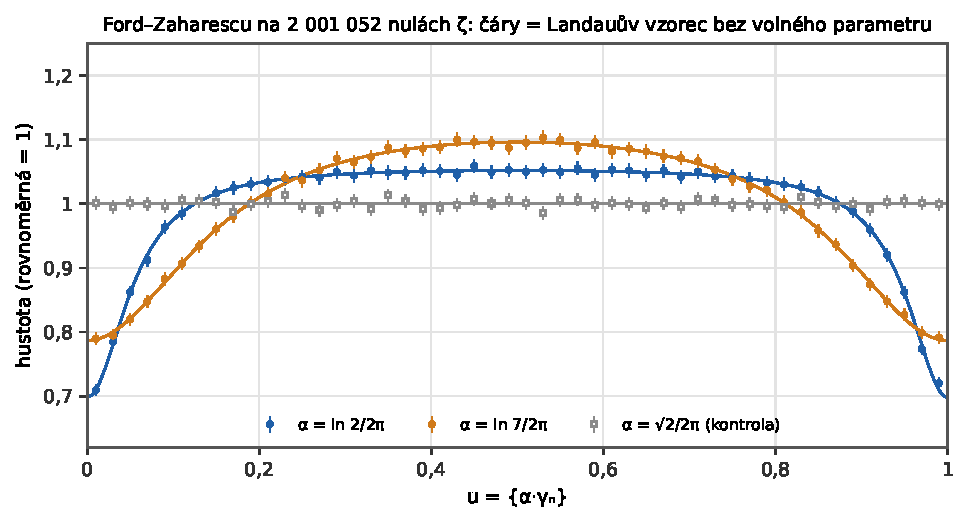
\includegraphics[width=0.88\textwidth,height=\textheight]{../../figures/09_ford_zaharescu_cz.pdf}
\caption{Obrázek 9. Hustota \(\{\alpha\gamma_n\}\) na 2 001 052 nulách
\(\zeta\) pro \(\alpha = \ln 2/2\pi\), \(\ln 7/2\pi\) a kontrolní
\(\sqrt2/2\pi\) (\(\pm 2\) chyby) s předpovědí z Landauova vzorce
(čáry).}
\end{figure}

\hypertarget{literatura}{%
\section{Literatura}\label{literatura}}
\small

\begin{enumerate}
\def\labelenumi{\arabic{enumi}.}
\tightlist
\item
  Hess, D. (2026). Berry saturation and the statistics of the Riemann
  zeros from \(t \approx 10^4\) to \(10^{21}\): a reproducible numerical
  study. Zenodo. \url{https://doi.org/10.5281/zenodo.23815328}
\item
  Hess, D. (2026). Beyond the diagonal approximation: pair correlation,
  form factor and resonances of the Riemann zeros from
  \(t \approx 10^4\) to \(10^{21}\) --- a reproducible numerical study
  II. Zenodo. \url{https://doi.org/10.5281/zenodo.23928017}
\item
  Hess, D. (2026). Low-lying zeros of 795,381 quadratic Dirichlet
  L-functions up to conductor \(10^{10}\): the ratios conjecture,
  consecutive families and the first zero --- a reproducible numerical
  study III. Zenodo. \url{https://doi.org/10.5281/zenodo.23991165}
\item
  Hess, D. (2026). Three-point correlation of the Riemann zeros at
  finite height: the ratios conjecture bin by bin on 147 million zeros
  up to \(t = 3\cdot10^{10}\), the amplitude of the deviation from GUE,
  and smaller sets further up --- a reproducible numerical study IV.
  Zenodo. \url{https://doi.org/10.5281/zenodo.24094318}
\item
  Conrey, J. B., Farmer, D. W., Keating, J. P., Rubinstein, M. O. \&
  Snaith, N. C. (2005). Integral moments of L-functions. Proc. London
  Math. Soc. 91, 33--104.
\item
  Keating, J. P. \& Snaith, N. C. (2000). Random matrix theory and
  L-functions at \(s = 1/2\). Commun. Math. Phys. 214, 91--110.
\item
  Jutila, M. (1981). On the mean value of \(L(1/2, \chi)\) for real
  characters. Analysis 1, 149--161.
\item
  Soundararajan, K. (2000). Nonvanishing of quadratic Dirichlet
  L-functions at \(s = 1/2\). Ann. of Math. 152, 447--488.
\item
  Diaconu, A., Goldfeld, D. \& Hoffstein, J. (2003). Multiple Dirichlet
  series and moments of zeta and L-functions. Compositio Math. 139,
  297--360.
\item
  Diaconu, A. \& Whitehead, I. (2021). On the third moment of
  \(L(1/2, \chi_d)\) II: the number field case. J. Eur. Math. Soc. 23,
  2051--2070. \url{https://doi.org/10.4171/JEMS/1049}
\item
  Alderson, M. W. \& Rubinstein, M. O. (2012). Conjectures and
  experiments concerning the moments of \(L(1/2, \chi_d)\). Exp. Math.
  21, 307--328. (arXiv:1110.0253)
\item
  Hough, B. (2015). The distribution of the logarithm in an orthogonal
  and a symplectic family of L-functions. Forum Math.
  \url{https://doi.org/10.1515/forum-2011-0105} (arXiv:1109.1783)
\item
  Gonek, S. M., Hughes, C. P. \& Keating, J. P. (2007). A hybrid
  Euler--Hadamard product for the Riemann zeta function. Duke Math. J.
  136, 507--549. \url{https://doi.org/10.1215/S0012-7094-07-13634-2}
\item
  Bui, H. M. \& Keating, J. P. (2008). On the mean values of L-functions
  in orthogonal and symplectic families. Proc. London Math. Soc. 96,
  335--366. \url{https://doi.org/10.1112/plms/pdm046}
\item
  Conrey, J. B., Farmer, D. W. \& Zirnbauer, M. R. (2008).
  Autocorrelation of ratios of L-functions. Commun. Number Theory Phys.
  2, 593--636.
\item
  Conrey, J. B. \& Snaith, N. C. (2007). Applications of the L-functions
  ratios conjectures. Proc. London Math. Soc. 94, 594--646.
\item
  Fazzari, A. (2024). A weighted one-level density of families of
  L-functions. Algebra Number Theory 18, 87--132.
  \url{https://doi.org/10.2140/ant.2024.18.87} (arXiv:2109.07244)
\item
  Sugiyama, S. \& Suriajaya, A. I. (2022). Weighted one-level density of
  low-lying zeros of Dirichlet L-functions. arXiv:2201.00326.
\item
  Lesesvre, D. \& Suriajaya, A. I. (2026). A connection between
  low-lying zeros and central values of L-functions. arXiv:2605.12688.
\item
  The PARI Group (2025). PARI/GP version 2.17.2.
  \url{https://pari.math.u-bordeaux.fr/}
\item
  Stopple, J. (2009). The quadratic character experiment. Exp. Math. 18,
  193--200. (arXiv:0802.4255)
\item
  Berry, M. V. (2001). Geometry of phase and polarization singularities
  illustrated by edge diffraction and the tides. Proc. SPIE 4403, 1--12.
  \url{https://doi.org/10.1117/12.428252}
\item
  Berry, M. V. \& Dennis, M. R. (2001). Knotted and linked phase
  singularities in monochromatic waves. Proc. R. Soc. Lond. A 457,
  2251--2263. \url{https://doi.org/10.1098/rspa.2001.0826}
\item
  Berry, M. V. \& Dennis, M. R. (2004). Quantum cores of optical phase
  singularities. J. Opt. A: Pure Appl. Opt. 6, S178--S180.
  \url{https://doi.org/10.1088/1464-4258/6/5/006}
\item
  Berry, M. V. (2005). Phase vortex spirals. J. Phys. A: Math. Gen.~38,
  L745--L751. \url{https://doi.org/10.1088/0305-4470/38/45/L01}
\item
  Berry, M. V. \& Goldberg, J. (1988). Renormalisation of curlicues.
  Nonlinearity 1, 1--26. \url{https://doi.org/10.1088/0951-7715/1/1/001}
\item
  Hess, D. (2026). Phase singularities of a windowed exponential sum
  over the Riemann zeros near the Landau--Gonek peak of \(p = 2\): an
  exploratory note (v1.1). Zenodo.
  \url{https://doi.org/10.5281/zenodo.24180562}
\item
  Ford, K. \& Zaharescu, A. (2005). On the distribution of imaginary
  parts of zeros of the Riemann zeta function. J. reine angew. Math.
  579, 145--158. (arXiv:math/0405459)
\item
  Ford, K., Soundararajan, K. \& Zaharescu, A. (2009). On the
  distribution of imaginary parts of zeros of the Riemann zeta function,
  II. Math. Ann. 343, 487--505.
  \url{https://doi.org/10.1007/s00208-008-0280-x}
\item
  Landau, E. (1911). Über die Nullstellen der Zetafunktion. Math. Ann.
  71, 548--564.
\end{enumerate}

\end{document}
